%definira klasu dokumenta 
\documentclass[12pt]{report} 

%prostor izmedu naredbi \documentclass i \begin{document} se zove uvod. U njemu se nalaze naredbe koje se odnose na cijeli dokument

%osnovni LaTex ne može riješiti sve probleme, pa se koriste različiti paketi koji olakšavaju izradu željenog dokumenta
\usepackage[croatian]{babel} 
\usepackage{amssymb}
\usepackage{amsmath}
\usepackage{txfonts}
\usepackage{mathdots}
\usepackage{titlesec}
\usepackage{array}
\usepackage{lastpage}
\usepackage{etoolbox}
\usepackage{tabularray}
\usepackage{color, colortbl}
\usepackage{adjustbox}
\usepackage{geometry}
\usepackage[classicReIm]{kpfonts}
\usepackage{hyperref}
\usepackage{fancyhdr}

\usepackage{float}
\usepackage{setspace}
\restylefloat{table}


\patchcmd{\chapter}{\thispagestyle{plain}}{\thispagestyle{fancy}}{}{} %redefiniranje stila stranice u paketu fancyhdr

%oblik naslova poglavlja
\titleformat{\chapter}{\normalfont\huge\bfseries}{\thechapter.}{20pt}{\Huge}
\titlespacing{\chapter}{0pt}{0pt}{40pt}


\linespread{1.3} %razmak između redaka

\geometry{a4paper, left=1in, top=1in,}  %oblik stranice

\hypersetup{ colorlinks, citecolor=black, filecolor=black, linkcolor=black,	urlcolor=black }   %izgled poveznice


%prored smanjen između redaka u nabrajanjima i popisima
\newenvironment{packed_enum}{
	\begin{enumerate}
		\setlength{\itemsep}{0pt}
		\setlength{\parskip}{0pt}
		\setlength{\parsep}{0pt}
	}{\end{enumerate}}

\newenvironment{packed_item}{
	\begin{itemize}
		\setlength{\itemsep}{0pt}
		\setlength{\parskip}{0pt}
		\setlength{\parsep}{0pt}
	}{\end{itemize}}




%boja za privatni i udaljeni kljuc u tablicama
\definecolor{LightBlue}{rgb}{0.9,0.9,1}
\definecolor{LightGreen}{rgb}{0.9,1,0.9}

%Promjena teksta za dugačke tablice
\DefTblrTemplate{contfoot-text}{normal}{Nastavljeno na idućoj stranici}
\SetTblrTemplate{contfoot-text}{normal}
\DefTblrTemplate{conthead-text}{normal}{(Nastavljeno)}
\SetTblrTemplate{conthead-text}{normal}
\DefTblrTemplate{middlehead,lasthead}{normal}{Nastavljeno od prethodne stranice}
\SetTblrTemplate{middlehead,lasthead}{normal}

%podesavanje zaglavlja i podnožja

\pagestyle{fancy}
\lhead{Programsko inženjerstvo}
\rhead{Ozdravi}
\lfoot{OZDRAVI-G11-T4}
\cfoot{stranica \thepage/\pageref{LastPage}}
\rfoot{\today}
\renewcommand{\headrulewidth}{0.2pt}
\renewcommand{\footrulewidth}{0.2pt}


\begin{document} 
	
	
	
	\begin{titlepage}
		\begin{center}
			\vspace*{\stretch{1.0}} %u kombinaciji s ostalim \vspace naredbama definira razmak između redaka teksta
			\LARGE Programsko inženjerstvo\\
			\large Ak. god. 2023./2024.\\
			
			\vspace*{\stretch{3.0}}
			
			\huge Ozdravi\\
			\Large Dokumentacija, Rev. \textit 1\\
			
			\vspace*{\stretch{12.0}}
			\normalsize
			Grupa: \textit{OZDRAVI-G11-T4}\\
			Voditelj: \textit{Hrvoje Cerin}\\
			
			
			\vspace*{\stretch{1.0}}
			Datum predaje: \textit{17. 11. 2023.}\\
	
			\vspace*{\stretch{4.0}}
			
			Nastavnik: \textit{mr. sc. Hrvoje Šimić}\\
		
		\end{center}

	
	\end{titlepage}

	
	\tableofcontents


	\chapter{Dnevnik promjena dokumentacije}

		\begin{longtblr}[
				label=none
			]{
				width = \textwidth, 
				colspec={|X[2]|X[13]|X[3]|X[3]|}, 
				rowhead = 1
			}
			\hline
			\textbf{Rev.}	& \textbf{Opis promjene/dodatka} & \textbf{Autori} & \textbf{Datum}\\[3pt] \hline
			0.1 & Napravljen predložak.	& Hrvoje Cerin & 8.11.2013. 		\\[3pt] \hline 
			0.2	& Dopisane upute za povijest dokumentacije.\newline Dodane reference. & * & 24.08.2013. 	\\[3pt] \hline 
			0.5 & Dodan \textit{Use Case} dijagram i jedan sekvencijski dijagram, funkcionalni i nefunkcionalni zahtjevi i dodatak A & * & 25.08.2013. \\[3pt] \hline 
			0.6 & Arhitektura i dizajn sustava, algoritmi i strukture podataka & Matko Ljepović & 16.11.2023. \\[3pt] \hline 
			0.8 & Povijest rada i trenutni status implementacije,\newline Zaključci i plan daljnjeg rada & * & 28.08.2013. \\[3pt] \hline 
			0.9 & Dodavanje opisa projektnog zadatka & Leon Tišljarić & 15.11.2023. \\[3pt] \hline 
			0.10 & Opisi obrazaca uporabe & Leon Tišljarić & 15.11.2023. \\[3pt] \hline 
			0.11 & Kreiranje dijagrama obrazaca uporabe & Leon Tišljarić & 17.11.2023. \\[3pt] \hline 
			0.12 & Kreiranje sekvencijskog dijagrama & Leon Tišljarić & 17.11.2013. \\[3pt] \hline 
			\textbf{1.0} & Verzija samo s bitnim dijelovima za 1. ciklus & Svi članovi tima & 17.11.2023. \\[3pt] \hline 
			&  &  & \\[3pt] \hline	
		\end{longtblr}
	

	\chapter{Opis projektnog zadatka}
		Cilj ovog projekta je razviti programsku podršku za stvaranje web aplikacije "Ozdravi" koja će služiti za povezivanje roditelja s medicinskim stručnjacima poput pedijatara i liječnika. Aplikacija ima za cilj olakšati komunikaciju, štedjeti vrijeme i ubrzati proces pregleda oboljele djece.
		
		Roditeljima će aplikacija omogućiti jednostavan pristup informacijama o zdravlju njihovog djeteta, uključujući povijest bolesti, preporuke liječnika te prijavu samih pregleda djeteta online putem. Liječnicima i pedijatrima će aplikacija pružiti bolji uvid u medicinsku povijest djece omogućujući im brže donošenje odluka, pregledavanje, planiranje i organizaciju pristiglih zahtjeva za pregled djece te slanje povratnih informacija i dokumenata roditeljima bez potrebe fizičkog posjeta roditelja za preuzimanje istih. Za administratorski pristup aplikaciji, omogućit će se širok spektar ovlasti kako bi administrator imao potpunu kontrolu i pristup svim podacima. Samim time administrator može nadzirati, otkriti i ukloniti nastale probleme jednostavnim putem te tako održavati web aplikaciju i pružati njezinim korisnicima brzu i efikasnu korisničku podršku. Sve zajedno će doprinijeti efikasnijem i transparentnijem procesu brige o zdravlju djece te olakšati život svi sudionika u tom procesu.
		
		Ciljana publika ove aplikacije su zauzeti, zaposleni roditelji s više djece koji su često na bolovanju zbog nemogućnosti interakcije između svih instanci u zdravstvu. Time su prisiljeni izostati iz posla, a djecu iz škole ili vrtića što uzrokuje stres i gubitak dragocjenog vremena čekajući po raznim natrpanim čekaonicama. Također, aplikacija je namijenjena liječnicima i pedijatrima koji žele olakšati svoj posao i povećati produktivnost. Korištenjem aplikacije oni ubrzavaju pregled dobivenih nalaza pacijenata, planiranje samog pregleda te slanje povratnih informacija roditeljima.
		
		\textbf{Neregistriranom korisniku} je omogućeno prijavljivanje u sustav s postojećim računom unosom lozinke i email adrese ili kreiranjem novog računa. Za kreiranje novog računa potrebni su sljedeći podaci: 
				\begin{packed_item}
					\item ime
					\item prezime
					\item spol
					\item datum rođenja
					\item adresa
					\item email
					\item lozinka
				\end{packed_item}
		
			\textbf{Roditeljima} je omogućeno pregledavanje naslovne stranice s novim obavijestima i zakazanim terminima pregleda, pregledavanje vlastitog profila, profila djece i povijesti pregleda, prijava željenog termina pregleda te slanje privatnih nalaza pregleda direktno liječniku/pedijatru.
		
		\textbf{Liječnicima/pedijatrim} je omogućeno pregledavanje dolaznih zahtjeva za preglede, popisa pacijenata, kreiranje novih zapisa pregleda, izdavanje ispričnica i molbi za bolovanje te brisanje i uređivanje prijašnjih pregleda pacijenata.
		
			\textbf{Administratorima} je omogućeno uređivanje osobnih podataka korisnika, brisanje samih korisnika, mijenjanje njihovih uloga, te brisanje i uređivanje pregleda pacijenata.
		
		Najpoznatija postojeća slična rješenja su ChARM Health i MyChart. MyChart je aplikacija razvijena od strane tvrtke Epic Systems Corporation, američke privatne tvrtke za razvoj softvera u području zdravstva. Ona pruža sigurnu online platformu koja omogućuje pacijentima pristup osobnim zdravstvenim informacijama i komunikaciju s njihovim zdravstvenim ustanovama. Neke od značajnijih zajedničkih stavki aplikacija Ozdravi i MyChart čine:
		
		\begin{packed_enum}
			\item Pristup medicinskim zapisima pacijenta
			\begin{itemize}
				\item mogućnost čuvanja i pregledavanja medicinske povijesti pacijenata
			\end{itemize}
			\item Zakazivanje termina
				\begin{itemize}
				\item omogućuju dogovor i zakazivanje termina pregleda slanjem upita liječniku
			\end{itemize}
			\item Pregled zdravstvenih profila
			\begin{itemize}
				\item mogućnost pohrane i pregleda korisničkih profila roditelja i djece
			\end{itemize}
			\item Izravno slanje medicinskih dokumenata
			\begin{itemize}
				\item pacijenti imaju mogućnost izravnog slanja novih nalaza zdravstvenoj ustanovi
			\end{itemize}
		\end{packed_enum}
		
		Nadalje, MyChart sadrži dodatne implementirane stavke koje nisu dio Ozdravi aplikacije:
		\begin{packed_enum}
			\item Stanje računa i plaćanje
			\begin{itemize}
				\item pacijenti mogu pregledavati i plaćati svoje medicinske račune
			\end{itemize}
			\item Integracija telekomunikacijskih tehnologija
			\begin{itemize}
				\item MyChart je integriran s telezdravstvenim uslugama omogućavajući pacijentima virtualne konzultacije
			\end{itemize}
			\item Podsjetnik o uzimanju ljekova
			\begin{itemize}
				\item aplikacija implementira praćenje doza uzimanih ljekova i dnevne podsjetnike o uzimanju istih
			\end{itemize}
		\end{packed_enum}

		\begin{figure}[H]
			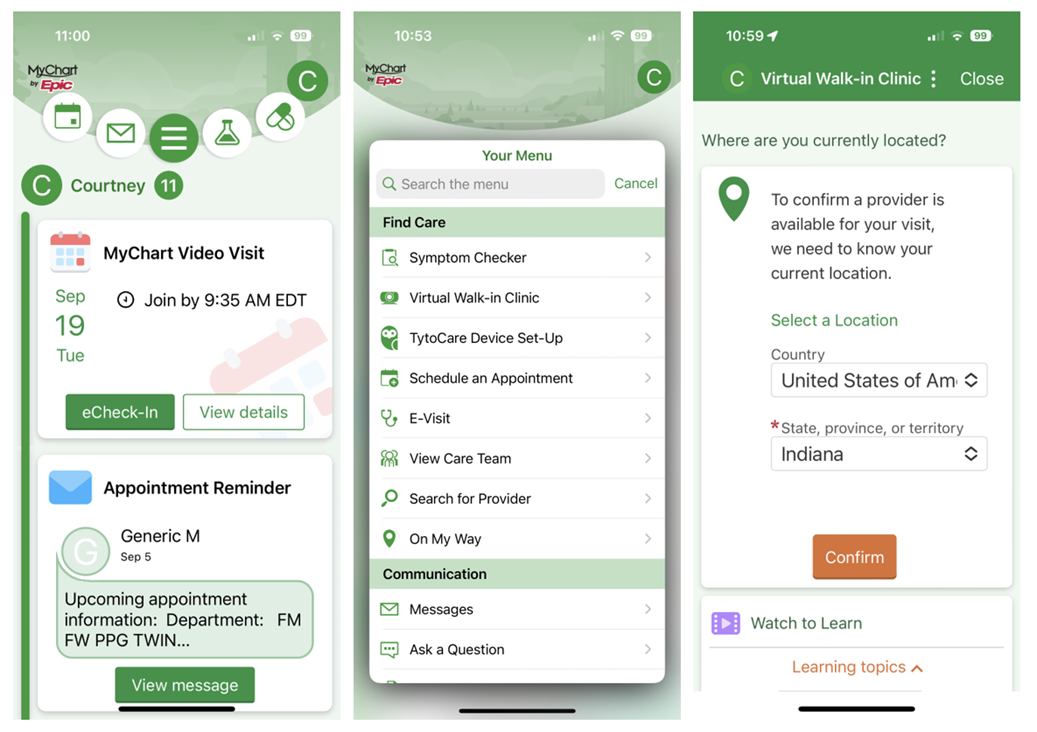
\includegraphics[scale=0.4]{slike/myChartMobileView.PNG}
			\centering
			\caption{MyChart mobilno sučelje}
			\label{fig:myChart}
		\end{figure}
		
		Projektni zadatak se nadalje može nadograditi dodavanjem:
		
		\begin{packed_item}
			\item geografskih mapa najbližih dostupnih zdravstvenih ustanova prilikom hitnih slučajeva
			\item forum portala za međusobnu komunikaciju svih korisnika aplikacije
			\item sustava za povratne informacije o iskustvima korisnika
			\item integracije s nosivim uređajima
			\item integracije s telezdravstvenim uslugama pojedinih zdravstvenih ustanova
			\item mogućnosti elektroničkih zahtjeva recepata
		\end{packed_item}
	\chapter{Specifikacija programske potpore}
		
	\section{Funkcionalni zahtjevi}
			\noindent \textbf{Dionici:}
			
			\begin{packed_enum}
				
				\item Roditelj
				\item Zdravstveni djelatnik	
				\begin{packed_enum}
					\item Liječnik
					\item Pedijatar
				\end{packed_enum}			
				\item Administrator
				\item Vanjski sudionik
				\begin{packed_enum}
					\item Poslodavac
					\item Škola/vrtić
				\end{packed_enum}
				\item Razvojni tim
			\end{packed_enum}
			
			\noindent \textbf{Aktori i njihovi funkcionalni zahtjevi:}
			
			
			\begin{packed_enum}
				\item  \underbar{Neregistrirani/neprijavljeni korisnik (inicijator) može:}
				
				\begin{packed_enum}
					\item se registrirati u sustav, stvoriti novi korisnički račun za koji su mu potrebni ime, prezime,  lozinka, e-mail adresa, spol, datum rođenja, adresa i OIB
				\item se prijaviti u sustav pomoću korisničkog računa i lozinke
				\end{packed_enum}
			
				\item  \underbar{Roditelj (inicijator) može:}
				\begin{packed_enum}
					\item vidjeti svoj profil i profile svoje djece
					\item pregledavati naslovnu stranicu s prikazom zakazanih termina i obavijestima od strane liječnika ili pedijatra
					\item prijaviti željeni termin pregleda ili poslati nalaze privatnih pregleda liječniku ili pedijatru
					\item pregledavati prijašnji popis bolesti i pregleda svoje djece
					\item odjaviti se iz aplikacije
				\end{packed_enum}
			
				\item  \underbar{Zdravstveni djelatnik (liječnik/pedijatar) (inicijator) može:}
				\begin{packed_enum}
					\item potvrditi ili odbiti zahtjev za pregledom dijeteta od strane roditelja
					\item vidjeti profil pacijenata te povijest pregleda i nalaza
					\item evidentirati preglede djece i događaje na istim
					\item poslati povratnu informaciju vezano uz nalaz roditelju
					\item pohraniti novi nalaz s povratnom informacijom
					\item izdati i odobriti ispričnicu u slučaju bolesti dijeteta
					\item preporučiti preporuku o bolovanju za roditelja bolesnog djeteta u slučaju pedijatra, a izdati i odobriti preporuku o bolovanju za roditelja bolesnog djeteta u slučaju liječnika
					\item odjaviti se iz aplikacije
				\end{packed_enum}
				
				\item  \underbar{Administrator (inicijator) može:}
				\begin{packed_enum}
					\item vidjeti popis svih korisnika i njihovih profila te profile njihove djece
					\item brisati i mijenjati razinu ovlasti korisnika aplikacije (roditelj, pedijatar/liječnik, administrator)
					\item dodati ili obrisati korisnika
					\item izmjeniti profile korisnika
					\item povezivati liječnike/pedijatre s roditeljima
					\item odjaviti se iz aplikacije
				\end{packed_enum}
				
				\item  \underbar{Vanjski sudionik (poslodavac/škola/vrtić) (sudionik) može:}
				\begin{packed_enum}
					\item zaprimiti ispričnicu/molbu za bolovanjem od strane liječnika/pedijatra
				\end{packed_enum}
			
				\item  \underbar{Baza podataka (sudionik) može:}
				\begin{packed_enum}
				\item pohranjuje sve podatke o korisnicima i njihovim ovlastima
				\item pohranjuje sve podatke o pregledima i bolestima pacijenata
				\item pohranjuje veze između liječnika/pedijatra i pacijenata
				\item pohranjuje zakazane termine i termine na čekanju za odobrenje
				\item pohranjuje ispričnice, preporuke o bolovanju i nalaze pacijenata
				\end{packed_enum}
			\end{packed_enum}
			
			\eject 
			
			
				
			\subsection{Obrasci uporabe}
				
				\subsubsection{Opis obrazaca uporabe}
				
					\noindent \underbar{\textbf{UC1 - Registriraj se}}
					\begin{packed_item}
	
						\item \textbf{Glavni sudionik: } Neregistrirani korisnik
						\item  \textbf{Cilj:} Kreirati korisnički račun za pristup sustavu
						\item  \textbf{Sudionici:} Baza podataka
						\item  \textbf{Preduvjet:} -
						\item  \textbf{Opis osnovnog tijeka:}
						
						\item[] \begin{packed_enum}
	
							\item Korisnik odabire opciju "Nemate račun? Registrirajte se!"
							\item Sustav vodi korisnika na putanju "/registracija" 
							\item Korisnik unosi potrebne podatke (ime, prezime, OIB, email, lozinku, potvrdu lozinke, spol, datum rođenja, adresu)
							\item Korisnik potvrđuje unos podataka odabirom akcije "Registriraj se"
							\item Sustav provjerava (ime, prezime, OIB, email, lozinku, potvrdu lozinke, spol, datum rođenja, adresu) i utvrđuje da je unos uspješan te vodi korisnika na naslovnu stranicu s putanjom "/naslovna"
						\end{packed_enum}
						
						\item  \textbf{Opis mogućih odstupanja:}
						
						\item[] \begin{packed_item}
							
							\item[5.a] Sustav radi provjere i utvrđuje da unos podataka nije uspješan te obavještava korisnika porukom. Sustav nastavlja izvođenje scenarija u koraku 3. 
	
							\item[5.b] Korisnik odabire opciju "Već imate račun? Prijavite se!" te ga sustav vodi na sučelje za prijavu na putanji "/prijava"
						
						\end{packed_item}
								
					\end{packed_item}
					
					
						\noindent \underbar{\textbf{UC2 - Prijavi se}}
					\begin{packed_item}
						
						\item \textbf{Glavni sudionik: }Korisnik
						\item  \textbf{Cilj:} Prijava u sustav s postojećim računom
						\item  \textbf{Sudionici:} Baza podataka
						\item  \textbf{Preduvjet:} Korisnik ima registrirani račun i nalazi se na putanji "/prijava"
						\item  \textbf{Opis osnovnog tijeka:}
						
						\item[] \begin{packed_enum}
							\item Korisnik unosi potrebne podatke (email, lozinku)
							\item Korisnik potvrđuje unos podataka odabirom akcije "Prijavi se"
							\item Sustav provjerava (email, lozinku) i utvrđuje da je unos uspješan te vodi korisnika na naslovnu stranicu s putanjom "/naslovna"
						\end{packed_enum}
						
						\item  \textbf{Opis mogućih odstupanja:}
						
						\item[] \begin{packed_item}
							
							\item[3.a] Sustav radi provjere i utvrđuje da prijava nije uspješan te obavještava korisnika porukom. Sustav nastavlja izvođenje scenarija u koraku 1. 
							
							\item[3.b] Korisnik odabire opciju "Nemate račun? Registrirajte se!" te ga sustav vodi na sučelje za registraciju na putanji "/registracija"							
						\end{packed_item}
						
					\end{packed_item}
					
					
				\noindent \underbar{\textbf{UC3 - Pregledaj naslovnu stranicu}}
				\begin{packed_item}
					
					\item \textbf{Glavni sudionik: }Roditelj, Administrator, Liječnik ili Pedijatar
					\item  \textbf{Cilj:} Pregled novih obavijesti i zakazanih termina od zadnje prijave
					\item  \textbf{Sudionici:} Baza podataka
					\item  \textbf{Preduvjet:} Korisnik sustava je prijavljen
					\item  \textbf{Opis osnovnog tijeka:}
					
					\item[] \begin{packed_enum}
						
						\item Korisnik odabire karticu "Naslovna" kod bočnog izbornika
						\item Sustav vodi korisnika na naslovnu stranicu s putanjom "/naslovna" i radi dohvaćanje potrebnih podataka (datum, vrijeme te ime, prezime, OIB medicinskog osoblja i dijeteta)
						\item Sustav prikazuje zakazene termine grupirane u sučelju "Zakazani termini", a nove obavijesti u sučelju "Nove obavijesti"
					\end{packed_enum}
					
						\item  \textbf{Opis mogućih odstupanja:}
					
					\item[] \begin{packed_item}
						
						\item[3.a] Sustav prilikom dohvaćanja podataka nailazi na grešku te obavještava korisnika porukom
						
						\item[3.b] Sustav prilikom dohvaćanja podataka utvrđuje da nema novih obavijesti ili zakazanih termina te obavještava korisnika porukom				
					\end{packed_item}
					
				\end{packed_item}
				
				
				\noindent \underbar{\textbf{UC4 - Pregledaj korisnički profil}}
				\begin{packed_item}
					
					\item \textbf{Glavni sudionik: }Roditelj, Administrator, Liječnik ili Pedijatar
					\item  \textbf{Cilj:} Pregled osobnih podataka korisnika i njegove dijece
					\item  \textbf{Sudionici:} Baza podataka
					\item  \textbf{Preduvjet:} Korisnik sustava je prijavljen
					\item  \textbf{Opis osnovnog tijeka:}
					
					\item[] \begin{packed_enum}
						\item Korisnik odabire karticu "Profil" kod bočnog izbornika
						\item Sustav vodi korisnika na stranicu s putanjom "/naslovna/profil"
						\item Sustav radi dohvaćanje podataka o korisniku (ime, prezime, OIB, spol, adresa, datum rođenja, email) i djeci (ime, prezime, OIB, spol, adresa, datum rođenja)
						\item Sustav prikazuje korisničke podatke grupirane u sučelju "MOJ PROFIL", a podatke o djeci grupirane u sučelju "PROFILI DJECE"
					\end{packed_enum}
					
					\item  \textbf{Opis mogućih odstupanja:}
					
					\item[] \begin{packed_item}
						
						\item[3.a] Korisnik sustava ima ulogu Administrator, Liječnik ili Pedijatar te sustav ne dohvaća podatke o dijeci
						\item[4.a] Korisnik sustava ima ulogu Roditelj i sustav ne prikazuje sučelje "PROFILI DJECE" nego obaviještava korisnika porukom da nema dijece
						\item[4.b] Korisnik sustava ima ulogu Administrator, Liječnik ili Pedijatar te sustav ne prikazuje sučelje "PROFILI DJECE"
					\end{packed_item}
					
				\end{packed_item}
				
				
				\noindent \underbar{\textbf{UC5 - Pregledaj popis povijesti pregleda i nalaza}}
				\begin{packed_item}
					
					\item \textbf{Glavni sudionik: }Roditelj, Liječnik ili Pedijatar
					\item  \textbf{Cilj:} Pregled popisa povijesti pregleda i nalaza djece/pacijenata
					\item  \textbf{Sudionici:} Baza podataka
					\item  \textbf{Preduvjet:} Korisnici sustava je prijavljen
					\item  \textbf{Opis osnovnog tijeka:}
					
					\item[] \begin{packed_enum}
						\item Korisnik s ulogom Roditelj odabire karticu "Popis pregleda" dok korisnik s ulogom Liječnik ili Pedijatar odabire karticu "Kartoni pacijenata" kod bočnog izbornika
						\item Sustav vodi korisnika na stranicu s putanjom "/naslovna/popisPregleda"
						\item Korisnik odabire željeno dijete iz padajućeg izbornika
						\item Na temelju odabira sustav radi dohvaćanje osnovnih podataka o prijašnjim pregledima (datum, vrijeme, ime, prezime, OIB i uloga medicinskog osoblja) i nalazima (datum, vrijeme, postojanje povratne informacije)
						\item Sustav u obliku liste prikazuje osnovne podatke o pregledima grupirane u sučelju "POVIJEST PREGLEDA", a osnovne podatke o nalazima u sučelju "POVIJEST NALAZA"
						\item Odabirom akcije "Otvori" sustav vodi korisnika na putanju "/naslovna/pregled/id" ili "/naslovna/nalaz/id"
					\end{packed_enum}
					
						\item  \textbf{Opis mogućih odstupanja:}
					
					\item[] \begin{packed_item}
						
						\item[4.a] Sustav prilikom dohvaćanja podataka nailazi na grešku te obavještava korisnika porukom
						
						\item[4.b] Sustav prilikom dohvaćanja podataka utvrđuje da dijete/pacijent nema prijašnjih pregleda ili nalaza te obavještava korisnika porukom					
					\end{packed_item}
					
				\end{packed_item}
				
				
				
				\noindent \underbar{\textbf{UC6 - Pregledaj odabrani pregled}}
				\begin{packed_item}
					
					\item \textbf{Glavni sudionik: }Roditelj, Liječnik ili Pedijatar
					\item  \textbf{Cilj:} Pregled svih informacija vezanih uz odabrani pregled
					\item  \textbf{Sudionici:} Baza podataka
					\item  \textbf{Preduvjet:} Sustav je obavio scenarij UC5
					\item  \textbf{Opis osnovnog tijeka:}
					
					\item[] \begin{packed_enum}
						\item Na temelju identifikatora "id" trenutne putanje "/naslovna/pregled/id" sustav radi dohvaćanje svih podataka o pregledu (datum, vrijeme, ime, prezime, OIB i uloga medicinskog osoblja, opis i trajanje simptoma, opis fizičkog pregleda, opis dijagnoze, propisani lijekovi, preporučeno daljnje liječenje, podaci o izdanoj ispričnici i preporuci o bolovanju) i dijetetu/pacijentu (ime, prezime, OIB, spol, adresa, datum rođenja)
						\item Sustav prikazuje dohvaćene podatke
						\item Korisnik akcijom "Preuzmi" preuzima ispričnicu i/ili preporuku za bolovanjem
					\end{packed_enum}
					
					\item  \textbf{Opis mogućih odstupanja:}
					
					\item[] \begin{packed_item}
						
						\item[1.a] Sustav prilikom dohvaćanja podataka nailazi na grešku te obavještava korisnika porukom
						
						\item[3.a] Sustav utvrđuje da nije izdana ispričnica i/ili preporuka o bolovanju i ne dozvoljava akciju "Preuzmi"			
					\end{packed_item}
					
				\end{packed_item}
				
				
				\noindent \underbar{\textbf{UC7 - Pregledaj odabrani nalaz}}
				\begin{packed_item}
					
					\item \textbf{Glavni sudionik: }Roditelj, Liječnik ili Pedijatar
					\item  \textbf{Cilj:} Pregled svih informacija vezanih uz odabrani nalaz
					\item  \textbf{Sudionici:} Baza podataka
					\item  \textbf{Preduvjet:} Sustav je obavio scenarij UC5
					\item  \textbf{Opis osnovnog tijeka:}
					
					\item[] \begin{packed_enum}
						\item Na temelju identifikatora "id" trenutne putanje "/naslovna/nalaz/id" sustav radi dohvaćanje svih podataka o nalazu (datum, vrijeme, nalaz, dodatna povratna informacija) i dijetetu/pacijentu (ime, prezime, OIB, spol, adresa, datum rođenja)
						\item Sustav prikazuje dohvaćene podatke
						\item Korisnik akcijom "Preuzmi" preuzima nalaz kao datoteku
					\end{packed_enum}
					
					\item  \textbf{Opis mogućih odstupanja:}
					
					\item[] \begin{packed_item}
						
						\item[1.a] Sustav prilikom dohvaćanja podataka nailazi na grešku te obavještava korisnika porukom	
					\end{packed_item}
					
				\end{packed_item}		
				
				
				
				
				\noindent \underbar{\textbf{UC8 - Pošalji novi zahtjev za termin pregleda}}
				\begin{packed_item}
					\item \textbf{Glavni sudionik: }Roditelj
					\item  \textbf{Cilj:} Poslati novi zahtjev za termin pregleda djeteta
					\item  \textbf{Sudionici:} Baza podataka, Liječnik, Pedijatar
					\item  \textbf{Preduvjet:} Roditelj je prijavljen u sustav i dijetetu je dodijeljeni liječnik ili pedijatar
					\item  \textbf{Opis osnovnog tijeka:}
					\item[] \begin{packed_enum}
						\item Roditelj odabire karticu "Novi Termin" kod bočnog izbornika
						\item Sustav vodi korisnika na stranicu s putanjom "/naslovna/noviTermin" i prikazuje formu za unos podataka o terminu pregleda
						\item Korisnik odabire željeno dijete i medicinsko osoblje iz padajućih izbornika
						\item Korisnik označava opciju "Želim zakazati termin"
						\item Sustav prikazuje dodatna polja za unos datuma i vremena
						\item Korisnik ispunjava polja i odabirom akcije "Pošalji" šalje podatke
						\item Sustav obrađuje podatke i porukom obavještava korisnika o uspješnom slanju
						
						\item[] \begin{packed_item}
						\item[3.a] Sustav prilikom dohvaćanja podataka nailazi na grešku te ne dozvoljava slanje novog termina pregleda
						
						\item[3.b] Sustav utvrđuje da dijete nema dodijeljenog liječnika i/ili pedijatra i ne dozvoljava slanje novog termina pregleda
						
						\item[7.a] Sustav prilikom obrade podataka obavještava korisnika da nisu popunjena sva obavezna polja porukom
						
						\item[7.b] Sustav prilikom slanja podataka nailazi na grešku te obavještava korisnika porukom o neuspješnom slanju	
					\end{packed_item}
				\end{packed_enum}
						
					\end{packed_item}
					
					
					
					\noindent \underbar{\textbf{UC9 - Pošalji novi nalaz dijeteta}}
					\begin{packed_item}
						
						\item \textbf{Glavni sudionik: }Roditelj
						\item  \textbf{Cilj:} Poslati i pohraniti novi nalaz
						\item  \textbf{Sudionici:} Baza podataka, Liječnik, Pedijatar
						\item  \textbf{Preduvjet:} Roditelj je prijavljen i ima dodijeljenu dijecu
						\item  \textbf{Opis osnovnog tijeka:}
						
						\item[] \begin{packed_enum}
							\item Roditelj odabire karticu "Novi Termin" kod bočnog izbornika
							\item Sustav vodi Roditelja na stranicu s putanjom "/naslovna/noviTermin" te prikazuje formu za prijenos nalaza
							\item Roditelj odabire željeno dijete i medicinsko osoblje iz padajućih izbornika
							\item Roditelj odabire opciju "Želim prenijeti nalaz"
							\item Sustav prikazuje dodatna polja za prijenos nalaza
							\item Roditelj prenosi nalaz akcijom "Odaberi datoteku"
							\item Roditelj traži povratnu informaciju odabirom opcije "Želim povratnu informaciju"
							\item Roditelj odabire akciju "Pošalji" za slanje nalaza
							\item Sustav obrađuje podatke i porukom obavještava korisnika o uspješnom slanju
						\end{packed_enum}
						
						\item  \textbf{Opis mogućih odstupanja:}
						
						\item[] \begin{packed_item}
							\item[3.a] Sustav prilikom dohvaćanja podataka nailazi na grešku te ne dozvoljava slanje novog nalaza
							
							\item[3.b] Sustav utvrđuje da dijete nema dodijeljenog liječnika i/ili pedijatra i ne dozvoljava slanje novog nalaza	
							
							\item[9.a] Sustav prilikom obrade podataka obavještava korisnika da nisu popunjena sva obavezna polja porukom
							
							\item[9.b] Sustav prilikom slanja podataka nailazi na grešku te obavještava korisnika porukom o neuspješnom slanju
						\end{packed_item}
					\end{packed_item}
					
					
					
					
					
					\noindent \underbar{\textbf{UC10 - Pošalji novi nalaz pacijenta}}
					\begin{packed_item}
						
						\item \textbf{Glavni sudionik: }Liječnik ili Pedijatar
						\item  \textbf{Cilj:} Poslati i pohraniti novi nalaz
						\item  \textbf{Sudionici:} Baza podataka, Roditelj
						\item  \textbf{Preduvjet:} Liječnik/Pedijatar je prijavljen i ima dodijeljene pacijente
						\item  \textbf{Opis osnovnog tijeka:}
						
						\item[] \begin{packed_enum}
							\item Liječnik/Pedijatar odabire karticu "Novi Nalaza" kod bočnog izbornika
							\item Sustav vodi Liječnika/Pedijatra na stranicu s putanjom "/naslovna/noviNalaz" te prikazuje formu za prijenos nalaza
							\item Liječnik/Pedijatar odabire željenog pacijenta iz padajućih izbornika
							\item Sustav prikazuje dodatna polja za prijenos nalaza
							\item Liječnik/Pedijatar prenosi nalaz akcijom "Odaberi datoteku"
							\item Liječnik/Pedijatar unosi povratnu informaciju u tekstualno polje
							\item Liječnik/Pedijatar odabire akciju "Pošalji" za slanje nalaza
							\item Sustav obrađuje podatke i porukom obavještava korisnika o uspješnom slanju
						\end{packed_enum}
						
						\item  \textbf{Opis mogućih odstupanja:}
						
						\item[] \begin{packed_item}
							\item[3.a] Sustav prilikom dohvaćanja podataka nailazi na grešku te ne dozvoljava slanje novog nalaza
							
							\item[3.b] Sustav utvrđuje da Liječnik/Pedijatar nema dodijeljenih pacijenata i ne dozvoljava slanje novog nalaza
							
							\item[8.a] Sustav prilikom obrade podataka obavještava korisnika da nisu popunjena sva obavezna polja porukom
							
							\item[8.b] Sustav prilikom slanja podataka nailazi na grešku te obavještava korisnika porukom o neuspješnom slanju
						\end{packed_item}
					\end{packed_item}
					
					
					
					
					\noindent \underbar{\textbf{UC11 - Otkaži zakazani termin}}
				\begin{packed_item}
					
					\item \textbf{Glavni sudionik: }Roditelj, Liječnik ili Pedijatar
					\item  \textbf{Cilj:} Otkazati zakazani termin
					\item  \textbf{Sudionici:} Baza podataka, Liječnik, Pedijatar, Roditelj
					\item  \textbf{Preduvjet:} Korisnik je prijavljen
					\item  \textbf{Opis osnovnog tijeka:}
					
					\item[] \begin{packed_enum}
						\item Roditelj odabire karticu "Novi Termin" dok Liječnik/Pedijatar odabire karticu "Termini na čekanju" kod bočnog izbornika
						\item Sustav vodi Roditelja na stranicu s putanjom "/naslovna/noviTermin" dok Liječnika/Pedijatra vodi na stranicu s putanjom "/naslovna/terminiNaCekanju"
						\item Sustav radi dohvaćanje podataka o zakazanim terminima (datum, vrijeme te ime, prezime, OIB medicinskog osoblja i dijeteta/pacijenta)
						\item Sustavu prikazuje zakazane termine grupirane u sučelju "ZAKAZANI TERMINI"
						\item Korisnik odabirom akcije "Otkaži" otkazuje određeni termin
						\item Sustav obrađuje podatke i micanjem termina iz sučelja obavještava korisnika o uspješnom otkazivanju termina
					\end{packed_enum}
					
					\item  \textbf{Opis mogućih odstupanja:}
					
					\item[] \begin{packed_item}
						\item[3.a] Sustav prilikom dohvaćanja podataka nailazi na grešku te obavještava korisnika porukom
						
						\item[3.b] Sustav prilikom dohvaćanja podataka otkriva da korisnik nema zakazanih termina te obavještava korisnika porukom
						
						\item[6.a] Sustav prilikom slanja podataka nailazi na grešku te ne briše odabrani termin iz sučelja
					\end{packed_item}
				\end{packed_item}				
							
							
							
							
				\noindent \underbar{\textbf{UC12 - Izbriši termin na čekanju}}
					\begin{packed_item}
						
						\item \textbf{Glavni sudionik: }Roditelj, Liječnik ili Pedijatar
						\item  \textbf{Cilj:} Obrisati termin na čekanju
						\item  \textbf{Sudionici:} Baza podataka, Liječnik, Pedijatar, Roditelj
						\item  \textbf{Preduvjet:} Korisnik je prijavljen
						\item  \textbf{Opis osnovnog tijeka:}
						
						\item[] \begin{packed_enum}
							\item Roditelj odabire karticu "Novi Termin" dok Liječnik/Pedijatar odabire karticu "Termini na čekanju" kod bočnog izbornika
							\item Sustav vodi Roditelja na stranicu s putanjom "/naslovna/noviTermin" dok Liječnika/Pedijatra vodi na stranicu s putanjom "/naslovna/terminiNaCekanju"
							\item Sustav radi dohvaćanje podataka o terminima na čekanju (datum, vrijeme te ime, prezime, OIB medicinskog osoblja i dijeteta/pacijenta)
							\item Sustavu prikazuje zakazane termine grupirane u sučelju "TERMINI NA ČEKANJU"
							\item Korisnik odabirom akcije "Izbriši" otkazuje određeni termin na čekanju dok to Liječnik/Pedijatar radi odabirom akcije "Odbij"
							\item Sustav obrađuje podatke i micanjem termina iz sučelja obavještava korisnika o uspješnom otkazivanju termina
						\end{packed_enum}
						
						\item  \textbf{Opis mogućih odstupanja:}
						
						\item[] \begin{packed_item}
							\item[3.a] Sustav prilikom dohvaćanja podataka nailazi na grešku te obavještava korisnika porukom
							
							\item[3.b] Sustav prilikom dohvaćanja podataka otkriva da korisnik nema termina na čekanju te obavještava korisnika porukom	
							
							\item[6.a] Sustav prilikom slanja podataka nailazi na grešku te ne briše odabrani termin iz sučelja
						\end{packed_item}
					\end{packed_item}		
					
					
					
				\noindent \underbar{\textbf{UC13 - Prihvati termin na čekanju}}
					\begin{packed_item}
						
						\item \textbf{Glavni sudionik: }Liječnik ili Pedijatar
						\item  \textbf{Cilj:} Prihvatiti termin na čekanju čime postaje zakazani termin
						\item  \textbf{Sudionici:} Baza podataka, Roditelj
						\item  \textbf{Preduvjet:} Liječnik/Pedijatar je prijavljen
						\item  \textbf{Opis osnovnog tijeka:}
						
						\item[] \begin{packed_enum}
							\item Liječnik/Pedijatar odabire karticu "Termini na čekanju" kod bočnog izbornika
							\item Sustav vodi Liječnika/Pedijatra na stranicu s putanjom "/naslovna/terminiNaCekanju"
							\item Sustav radi dohvaćanje podataka o terminima na čekanju (datum, vrijeme te ime, prezime, OIB medicinskog osoblja i pacijenta)
							\item Sustavu prikazuje zakazane termine grupirane u sučelju "TERMINI NA ČEKANJU"
							\item Liječnik/Pedijatar odabirom akcije "Prihvati" potvrđuje određeni termin
							\item Sustav obrađuje podatke i micanjem termina iz sučelja obavještava korisnika o uspješnom potvrđivanju termina čime postaje zakazani
						\end{packed_enum}
						
						\item  \textbf{Opis mogućih odstupanja:}
						
						\item[] \begin{packed_item}
							\item[3.a] Sustav prilikom dohvaćanja podataka nailazi na grešku te obavještava korisnika porukom
						
							\item[3.b] Sustav prilikom dohvaćanja podataka otkriva da nema termina na čekanju te obavještava korisnika porukom
							
							\item[6.a] Sustav prilikom slanja podataka nailazi na grešku te ne briše odabrani termin iz sučelja
						\end{packed_item}
					\end{packed_item}	
					
					
					
					
				\noindent \underbar{\textbf{UC14 - Dodaj povratnu informaciju nalazu}}
					\begin{packed_item}
						
						\item \textbf{Glavni sudionik: }Liječnik ili Pedijatar
						\item  \textbf{Cilj:} Dodati povratnu informaciju medicinskog osoblja o nalazu ako je Roditelj to zatražio
						\item  \textbf{Sudionici:} Baza podataka, Roditelj
						\item  \textbf{Preduvjet:} Liječnik/Pedijatar je prijavljen
						\item  \textbf{Opis osnovnog tijeka:}
						
						\item[] \begin{packed_enum}
							\item Liječnik/Pedijatar odabire karticu "Novi Nalaz" kod bočnog izbornika
							\item Sustav vodi Liječnika/Pedijatra na stranicu s putanjom "/naslovna/noviNalaz"
							\item Sustav radi dohvaćanje podataka o nalazima koji čekaju povratnu informaciju trenutno prijavljenog Liječnika/Pedijatra (datum, vrijeme, ime, prezime, OIB pacijenta, datoteku nalaza)
							\item Sustavu prikazuje nalaze grupirane u sučelju "NALAZI NA ČEKANJU"
							\item Liječnik/Pedijatar odabirom akcije "Više" prikazuje dodatna polja
							\item Odabirom akcije "Preuzmi" Liječnik/Pedijatar preuzima nalaz
							\item Liječnik/Pedijatar unosi povratnu informaciju u tekstualno polje
							\item Odabirom akcije "Pošalji" sustav šalje nalaz
							\item Sustav obrađuje podatke i porukom obavještava korisnika o uspješnom slanju povratne informacije za nalaz
						\end{packed_enum}
						
						\item  \textbf{Opis mogućih odstupanja:}
						
						\item[] \begin{packed_item}
							\item[3.a] Sustav prilikom dohvaćanja podataka nailazi na grešku te obavještava korisnika porukom
							
							\item[3.b] Sustav prilikom dohvaćanja podataka otkriva da nema nalaza na čekanju te obavještava korisnika porukom
							
							\item[9.a] Sustav prilikom slanja podataka nailazi na grešku te ne briše odabrani termin iz sučelja
						\end{packed_item}
					\end{packed_item}		
					
					
					
					
				\noindent \underbar{\textbf{UC15 - Dodaj novi pregled}}
					\begin{packed_item}
						
						\item \textbf{Glavni sudionik: }Liječnik ili Pedijatar
						\item  \textbf{Cilj:} Pohraniti podatke o pregledu pacijenta prilikom njegovog trajanja
						\item  \textbf{Sudionici:} Baza podataka, Roditelj
						\item  \textbf{Preduvjet:} Liječnik/Pedijatar je prijavljen
						\item  \textbf{Opis osnovnog tijeka:}
						
						\item[] \begin{packed_enum}
							\item Liječnik/Pedijatar odabire karticu "Novi Pregled" kod bočnog izbornika
							\item Sustav vodi Liječnika/Pedijatra na stranicu s putanjom "/naslovna/noviPregled"
							\item Sustav radi dohvaćanje podataka o zakazanim terminima Liječnika/Pedijatra (datum, vrijeme, ime, prezime, OIB pacijenta)
							\item Sustavi prikazuje formu s izborom trenutnog zakazanog termina
							\item Liječnik/Pedijatar odabire zakazani termin s padajućeg izbornika
							\item Sustav radi dohvaćanje podataka o pacijentu vezanom za taj termin (ime, prezime, OIB, spol, adresa, datum rođenja)
							\item Sustavu prikazuje dodatna tekstualna polja za ispunu (opis i trajanja simptoma, opis fizičkog pregleda, opis dijagnoze, propisani lijekovi, daljnji tretmani) i opciju za izdavanje ispričnice i preporuke o bolovanju
							\item Liječnik/Pedijatar popunjuje polja podacima
							\item Liječnik/Pedijatar odabire opciju "Izdaj ispričnicu"
							\item Sustav prikazuje dodatno polja za unos (naziv bolesti i datume odsudstva) te tekstualni prikaz ispričnice
							\item Liječnik/Pedijatar odabire opciju "Izdaj preporuku za bolovanje"
							\item Sustav prikazuje dodatni tekstualni prikaz preporuke za bolovanje
							\item Odabirom akcije "Pohrani" sustav sprema podatke o pregledu 
							\item Sustav obrađuje podatke i porukom obavještava korisnika o uspješnom spremanju nalaza
						\end{packed_enum}
						
						\item  \textbf{Opis mogućih odstupanja:}
						
						\item[] \begin{packed_item}
							\item[3.a] Sustav prilikom dohvaćanja podataka nailazi na grešku te obavještava korisnika porukom
							
							\item[3.b] Sustav prilikom dohvaćanja podataka otkriva da nema zakazanih termina  te obavještava korisnika porukom i ne dozvoljava unos podataka
							
							\item[3.a] Sustav prilikom dohvaćanja podataka nailazi na grešku te obavještava korisnika porukom
							
							\item[14.a] Sustav prilikom obrade podataka obavještava korisnika da nisu popunjena sva obavezna polja porukom
							
							\item[14.b] Sustav prilikom slanja podataka nailazi na grešku te obavještava korisnika porukom
							
						\end{packed_item}
					\end{packed_item}		
					
					
					
					
					\noindent \underbar{\textbf{UC16 - Odbij preporuku za bolovanje}}
					\begin{packed_item}
						
						\item \textbf{Glavni sudionik: }Liječnik
						\item  \textbf{Cilj:} Odbiti preporuku za bolovanje roditelja poslanu od strane Pedijatra
						\item  \textbf{Sudionici:} Baza podataka, Pedijatar
						\item  \textbf{Preduvjet:} Liječnik je prijavljen u sustav
						\item  \textbf{Opis osnovnog tijeka:}
						
						\item[] \begin{packed_enum}
							\item Liječnik odabire karticu "Preporuke za bolovanje"
							\item Sustav vodi Liječnika na stranicu s putanjom "/naslovna/preporukeZaBolovanje"
							\item Sustav radi dohvaćanje podataka o preporukama za bolovanje na čekanju za odobrenje od strane trenutno prijavljenog Liječnika (ime, prezime, OIB pedijatra i pacijenta, naziv dijagnoze, početak i kraj bolovanja pacijenta)
							\item Sustavu prikazuje zakazane termine grupirane u sučelju "PREPORUKE ZA BOLOVANJE NA ČEKANJU"
							\item Liječnik odabirom akcije "Odbij" odbija određenu preporuku za bolovanje roditelja tog pacijenta
							\item Sustav obrađuje podatke i micanjem preporuke iz sučelja obavještava korisnika o uspješnom otkazivanju termina
						\end{packed_enum}
						
						\item  \textbf{Opis mogućih odstupanja:}
						
						\item[] \begin{packed_item}
							\item[3.a] Sustav prilikom dohvaćanja podataka nailazi na grešku te obavještava korisnika porukom
							
							\item[3.b] Sustav prilikom dohvaćanja podataka otkriva da korisnik nema preporuka na čekanju te obavještava korisnika porukom
							
							\item[6.a] Sustav prilikom slanja podataka nailazi na grešku te ne briše odabranu preporuku iz sučelja
						\end{packed_item}
					\end{packed_item}	
					
					
					
					
				\noindent \underbar{\textbf{UC17 - Prihvati preporuku za bolovanje}}
					\begin{packed_item}
						
						\item \textbf{Glavni sudionik: }Liječnik
						\item  \textbf{Cilj:} Prihvatiti preporuku za bolovanje roditelja poslanu od strane Pedijatra
						\item  \textbf{Sudionici:} Baza podataka, Pedijatar
						\item  \textbf{Preduvjet:} Liječnik je prijavljen u sustav
						\item  \textbf{Opis osnovnog tijeka:}
						
						\item[] \begin{packed_enum}
							\item Liječnik odabire karticu "Preporuke za bolovanje"
							\item Sustav vodi Liječnika na stranicu s putanjom "/naslovna/preporukeZaBolovanje"
							\item Sustav radi dohvaćanje podataka o preporukama za bolovanje na čekanju za odobrenje od strane trenutno prijavljenog Liječnika (ime, prezime, OIB pedijatra i pacijenta, naziv dijagnoze, početak i kraj bolovanja pacijenta)
							\item Sustavu prikazuje zakazane termine grupirane u sučelju "PREPORUKE ZA BOLOVANJE NA ČEKANJU"
							\item Liječnik odabirom akcije "Prihvati" prihvaća određenu preporuku za bolovanje roditelja tog pacijenta
							\item Sustav obrađuje podatke i micanjem preporuke iz sučelja obavještava korisnika o uspješnom otkazivanju termina
						\end{packed_enum}
						
						\item  \textbf{Opis mogućih odstupanja:}
						
						\item[] \begin{packed_item}
							\item[3.a] Sustav prilikom dohvaćanja podataka nailazi na grešku te obavještava korisnika porukom
							
							\item[3.b] Sustav prilikom dohvaćanja podataka otkriva da korisnik nema preporuka na čekanju te obavještava korisnika porukom
							
							\item[6.a] Sustav prilikom slanja podataka nailazi na grešku te ne briše odabranu preporuku iz sučelja
						\end{packed_item}
					\end{packed_item}		
					
					
					
					
					\noindent \underbar{\textbf{UC17 - Odjavi se}}
					\begin{packed_item}
						
						\item \textbf{Glavni sudionik: }Roditelj, Administrator, Liječnik ili Pedijatar
						\item  \textbf{Cilj:} Korisnik se odjavljuje iz sustava
						\item  \textbf{Sudionici:} Baza podataka
						\item  \textbf{Preduvjet:} Korisnik aplikacije je prijavljen u sustav
						\item  \textbf{Opis osnovnog tijeka:}
						
						\item[] \begin{packed_enum}
							
							\item Korisnik odabire karticu "Odjava" kod bočnog izbornika
							\item Sustav obrađuje podatke i vodi korisnika na stranicu prijave s putanjom "/prijava prilikom uspješne odjave
						\end{packed_enum}
						
						\item  \textbf{Opis mogućih odstupanja:}
						
						\item[] \begin{packed_item}
							\item[2.a] Sustav prilikom slanja podataka nailazi na grešku te vodi korisnika na stranicu prijave s putanjom "/prijava nego korisnik ostaje prijavljen
						\end{packed_item}
						
					\end{packed_item}
					

											
				\noindent \underbar{\textbf{U18 - Uređivanje korisničkog profila}}
				\begin{packed_item}
					
					\item \textbf{Glavni sudionik: }Administrator
					\item  \textbf{Cilj:} : Uređivati korisnički profili izmjenom njegovih podataka
					\item  \textbf{Sudionici:} Baza podataka
					\item  \textbf{Preduvjet:} Administrator je prijavljen u sustav
					\item  \textbf{Opis osnovnog tijeka:}
					
					\item[] \begin{packed_enum}						
						\item Administrator odabire karticu "Upravljanje računima" kod bočnog izbornika
						\item Sustav vodi Administratora na stranicu s putanjom "/naslovna/upravljanjeRacunima"
						\item Sustav prikazuje formu s poljem za unos OIB-a željenog korisnika
						\item Administrator unosi OIB
						\item Sustav radi dohvaćanje podataka o korisniku na temelju OIB-a (ime, prezime, OIB, spol, adresa, datum rođenja, email, uloga) i prikazuje dodatnu formu s poljima za uređivanje podataka
						\item Administrator uređuje podatke
						\item Administrator odabirom akcije "Potvrdi" pohranjuje unesene promjene 
						\item Sustav obrađuje podatke i porukom obavještava Adminstratora o uspješnoj promjeni podataka
						\end{packed_enum}	
					
					\item  \textbf{Opis mogućih odstupanja:}
					
					\item[] \begin{packed_item}
						\item[5.a] Sustav prilikom dohvaćanja podataka nailazi na grešku te obavještava korisnika porukom
						\item[8.a] Sustav prilikom slanja podataka nailazi na grešku te obavještava korisnika porukom
					\end{packed_item}
					
				\end{packed_item}	
				
				
				
				
				\noindent \underbar{\textbf{U18 - Brisanje korisničkog profila}}
				\begin{packed_item}
					
					\item \textbf{Glavni sudionik: }Administrator
					\item  \textbf{Cilj:} : Izbrisati korisnički profili iz sustava
					\item  \textbf{Sudionici:} Baza podataka
					\item  \textbf{Preduvjet:} Administrator je prijavljen u sustav
					\item  \textbf{Opis osnovnog tijeka:}
					
					\item[] \begin{packed_enum}						
						\item Administrator odabire karticu "Upravljanje računima" kod bočnog izbornika
						\item Sustav vodi Administratora na stranicu s putanjom "/naslovna/upravljanjeRacunima"
						\item Sustav prikazuje formu s poljem za unos OIB-a željenog korisnika
						\item Administrator unosi OIB
						\item Sustav radi dohvaćanje podataka o korisniku na temelju OIB-a (ime, prezime, OIB, spol, adresa, datum rođenja, email, uloga) i prikazuje dodatnu formu s poljima za uređivanje podataka
						\item Administrator odabirom akcije "Izbriši profil" briše korisnički profil
						\item Sustav obrađuje podatke i porukom obavještava Adminstratora o uspješnom brisanju profila
					\end{packed_enum}	
					
					\item  \textbf{Opis mogućih odstupanja:}
					
					\item[] \begin{packed_item}
						\item[5.a] Sustav prilikom dohvaćanja podataka nailazi na grešku te obavještava korisnika porukom
						\item[8.a] Sustav prilikom slanja podataka nailazi na grešku te obavještava korisnika porukom
					\end{packed_item}
					
				\end{packed_item}					
				
			
					
				\subsubsection{Dijagrami obrazaca uporabe}
					
				\begin{figure}[H]
					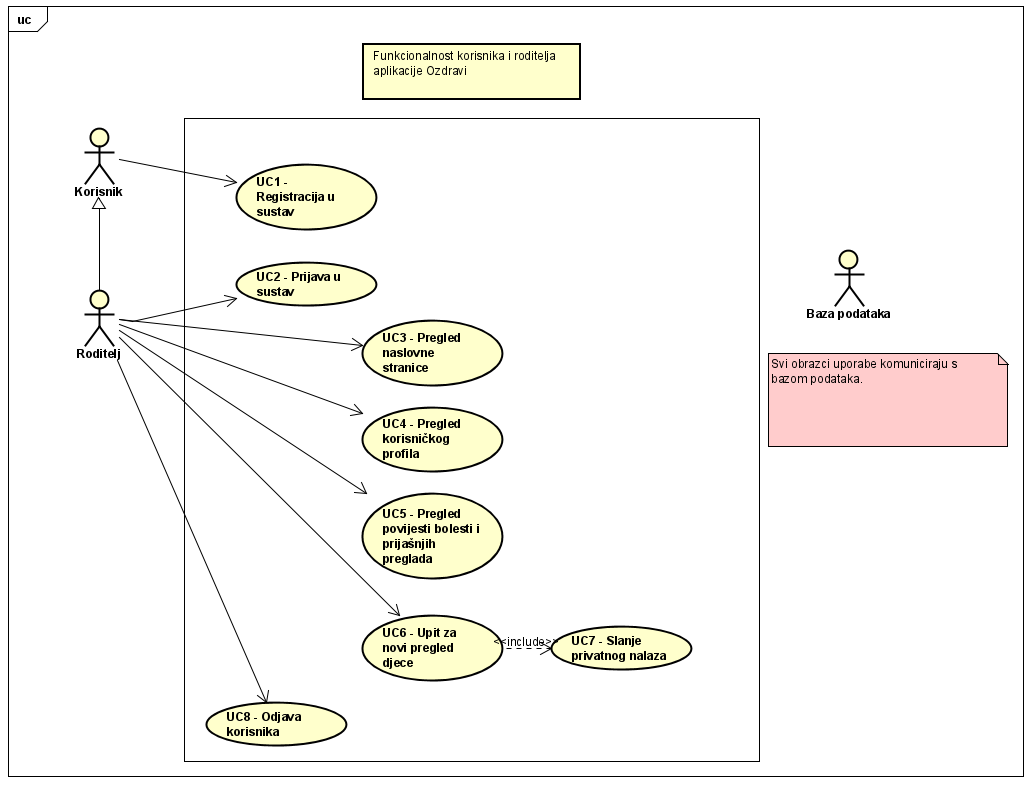
\includegraphics[scale=0.6]{dijagrami/UCRoditelj.PNG}
					\centering
					\caption{Dijagram obrasca uporabe, funkcionalnost korisnika i roditelja}
					\label{fig:myChart}
				\end{figure}
				
				\begin{figure}[H]
					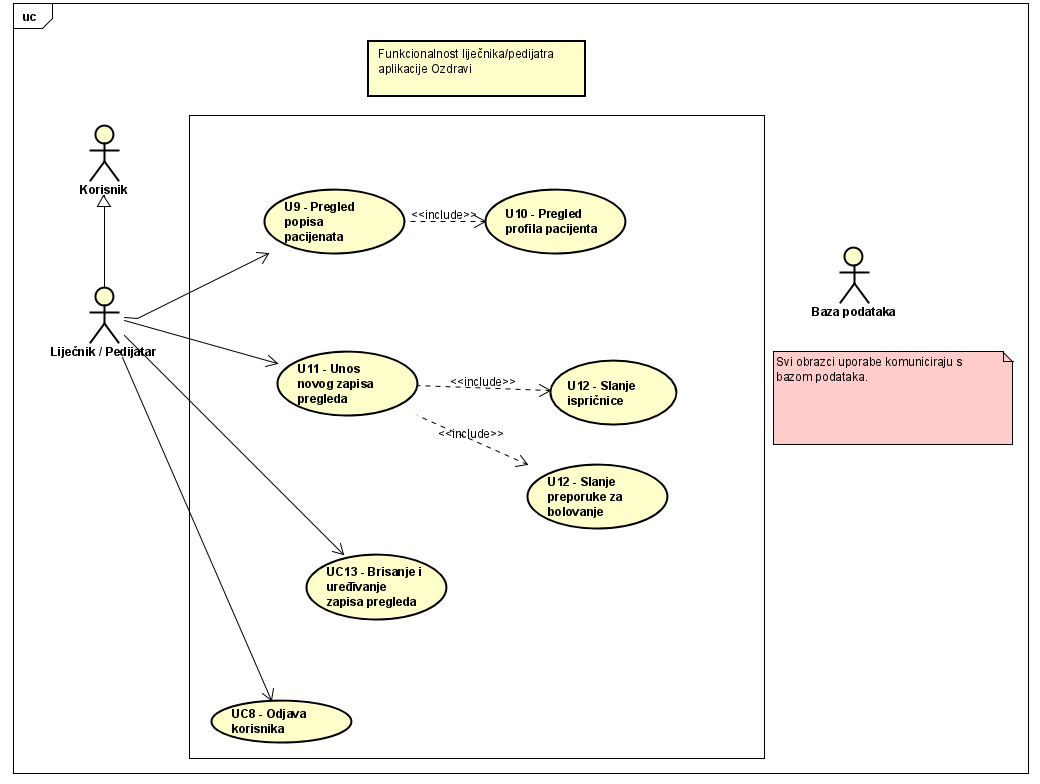
\includegraphics[scale=0.6]{dijagrami/UCLijecnikPedijatar.PNG}
					\centering
					\caption{Dijagram obrasca uporabe, funkcionalnost liječnika/pedijatra}
					\label{fig:myChart}
				\end{figure}
				
				\begin{figure}[H]
					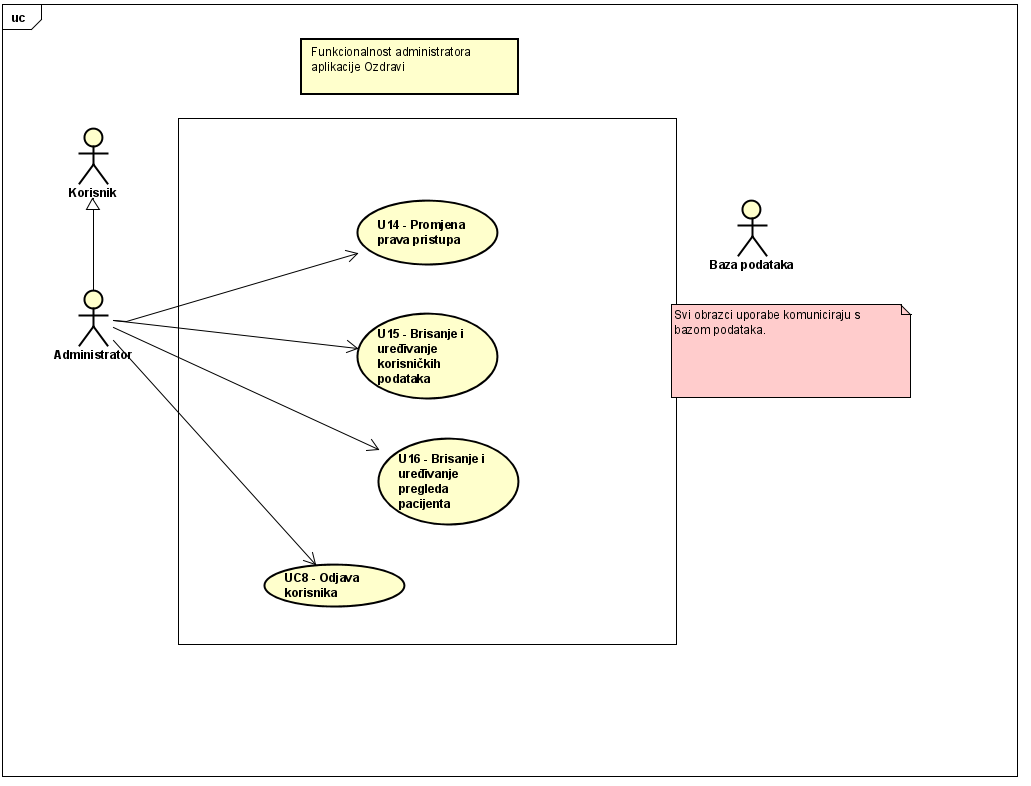
\includegraphics[scale=0.6]{dijagrami/UCAdministrator.PNG}
					\centering
					\caption{Dijagram obrasca uporabe, funkcionalnost administratora}
					\label{fig:myChart}
				\end{figure}
				
			\subsection{Sekvencijski dijagrami}
				
				\subsubsection{Obrazac uporabe U2 - Registracija korisnika}
				Klijent dolazi na stranicu registracije i unosi potrebne podatke za kreiranje računa (ime, prezime, OIB, datum rođenja, adresa, spol, email, lozinka). Ako uneseni podaci ne zadovoljavaju određeni format, javlja se greška o neispravnom formatu, a gumb registracije ostaje neaktivan. Nakon što korisnik unese sve podatke ispravno, omogućava se gumb registracije i šalje se zahtjev za spremanje u bazu podataka. Ako već postoji korisnik s istim emailom ili OIB-om, registracija je neuspješna i opet se javlja greška korisniku. Tek nakon što se unesu OIB i email koji nisu već registrirani, registracija postaje uspješna i korisnik se preusmjerava na naslovnu stranicu.
				
				\begin{figure}[H]
					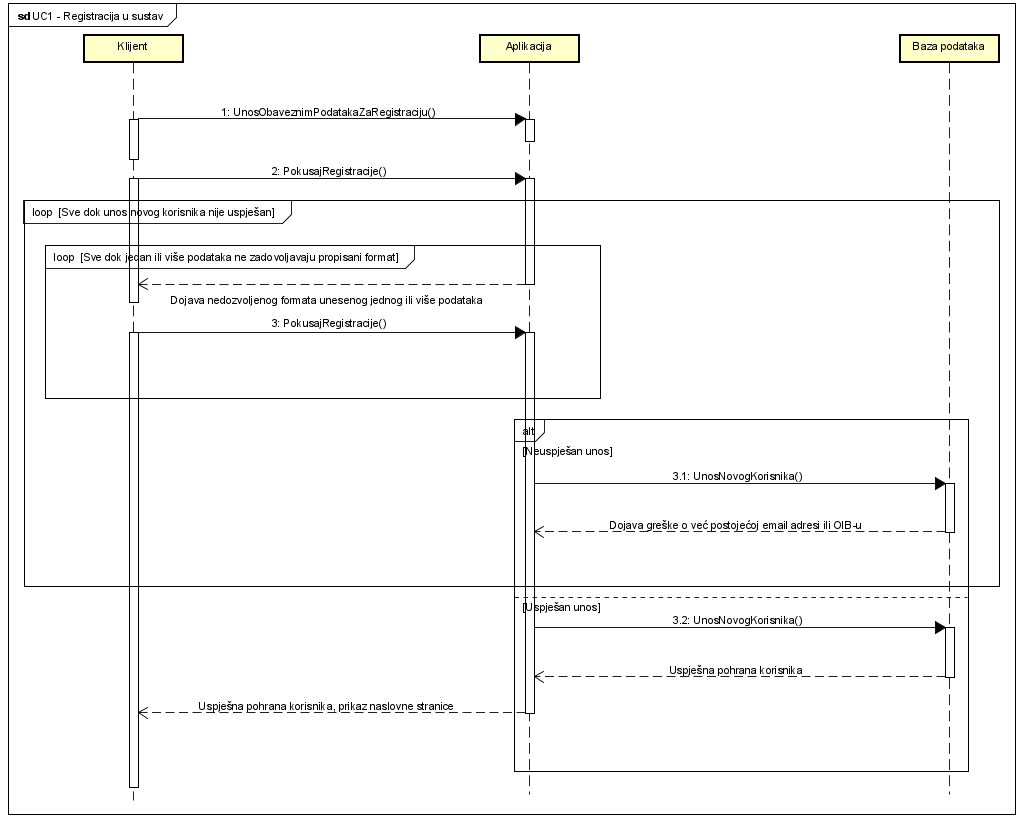
\includegraphics[scale=0.6]{dijagrami/SDRegistracija.PNG}
					\centering
					\caption{Sekvencijski dijagram za UC2}
					\label{fig:myChart}
				\end{figure}
	
		\section{Ostali zahtjevi}
			\begin{packed_item}
			\item	Sustav treba omoguciti rad više korisnika u stvarnom vremenu
			\item	Korisničko sučelje i sustav moraju podržavati hrvatsku abecedu
			\item	Izvršavanje dijela programa u kojem se pristupa bazi podataka ne smije trajati duze od nekoliko sekundi
			\item	Neispravno koristenje korisničkog sučelja ne smije narušiti funkcionalnost i rad sustava
			\item	Sustav treba biti jednostavan za koristenje
			\item	Nadogradnja sustava ne smije narusavati postojeće funkcionalnosti sustava
			\item	Veza s bazom podataka mora biti kvalitetno zastičena, brza i otporna na vanjske greške
			\item	Pristup sustavu mora biti omogucen iz javne mreže pomoću HTTPS
			\end{packed_item}
			 
			 
			 
	

	\chapter{Arhitektura i dizajn sustava}

		\noindent\textit{Arhitektura se može podijeliti na 3 djela: }
		\begin{packed_item}
			\item \textbf{Korisničko sučelje(frontend)} Predstavlja sve što korisnik vidi. Prikazuje korisničko sučelje, prenosi podatke od korisnika na backend i obrnuto.
			\item \textbf{Aplikacijski sloj(backend)}
			Bavi se procesiranje podataka koje korisnik zatraži preko frontenda. Obrađuje i validira podatke, te pohranjuje i dohvaća podatke iz baze.
			\item \textbf{Baza podataka}
			U bazu podataka se spremaju svi podatci. Služi za lakše spremanje, dohvaćanje i održavanje integriteta podadtaka.
		\end{packed_item}
		
	
		
		\noindent Backend dio aplikacije je rađen u javi korištenjem spring boot alata. Dok je frontend rađen u react-u, proramskim jezikom javascript. Za razvojno okruženje frontenda korišten je Microsoft visual studio, a za backend IntelliJ IDEA. Arhitektura susava temeljena je na MVC(Model-View-Controller) modelu. Prednost takve arhitekture je što su komponente neovisne te mogu biti testirane zasebno što olakšava proširivanje, testiranje i održavanje aplikacije.
		
		\begin{packed_item}
	\item \textbf{Model} Predstavlja poslovnu logiku i podatke aplikacije. Ovdje se definiraju objekti i logika koji se koriste za dohvaćanje, ažuriranje i pohranu podataka. Ne ovisi o korisničkom sučelju.
	\item \textbf{View)}
	Predstavlja korisničko sučelje i odgovoran je za prikaz podataka. Ne sadrži poslovnu logiku i ne komunicira izravno s Modelom. Ažurira se na temelju promjena u Modelu.
	\item \textbf{Controller}
	Obradjuje korisničke zahtjeve i ažurira Model te odabire pravi View za prikaz. Glavna uloga je upravljati komunikacijom između Modela i Viewa. Ovisno o korisničkom zahtjevu, Controller može ažurirati Model, ažurirati View ili oboje.
\end{packed_item}
		

				
		\section{Baza podataka}
	Baza podataka služi nam za jednostavniju i bržu pohranu i dohvat podataka. Za našu aplikaciju koristili smo relacijsku bazu podataka. Osnovna struktura baze su povezane tablice koje su određene imenom i skupom atributa. Baza podataka sastoji se od sljedećih tablica: 
		
		\begin{packed_item}
			\item {Users}
			\item {Children}
			\item {ChildRegister}
			\item {ChildExaminations}
			\item {MedicalCertificates}
			\item {TestResults}
			\item {Notifications}
			\item {SpecialistAppointments}
			\item {VisitHistory}
		\end{packed_item}
		
			\subsection{Opis tablica}
			

		\noindent \textbf{User} entitet sastoji se od atributa: ID, userName, password, firstName, lastName, email, role. Entitet sadrži sve atribute vezane za korisnike koji su nam potrebni u izradi aplikacije. Ovaj entitet je u vezi Many-to-Many s entitetom Children preko ID atributa korisnika, One-to-Many vezom s entitetom Notifications preko atributa ID korisnik, One-to-Many vezom s entitetom SpecialistAppointments preko atributa ID korisnika, One-to-Many vezom s entitetom VisitHistory preko atributa ID korisnika i One-to-Many vezom s entitetom ChildExaminations preko atributa ID korisnika.
				
				
				\begin{longtblr}[
					label=none,
					entry=none
					]{
						width = \textwidth,
						colspec={|X[6,l]|X[6, l]|X[20, l]|}, 
						rowhead = 1,
					} %definicija širine tablice, širine stupaca, poravnanje i broja redaka naslova tablice
					\hline \SetCell[c=3]{c}{\textbf{Users}}	 \\ \hline[3pt]
					\SetCell{LightGreen}ID & INT	&  	Jedinstven identifikator korisnika 	\\ \hline
					userName	& VARCHAR & jedinstven naziv korisnika   	\\ \hline 
					password & VARCHAR & lozinka  \\ \hline 
					firstName & VARCHAR	& ime korisnika 		\\ \hline 
					lastName	& VARCHAR & prezime korisnika  	\\ \hline 
					email & VARCHAR & e-mail adresa korisnika \\ \hline
					role & VARCHAR & uloga korisnika \\ \hline
				\end{longtblr}
				
			\noindent \textbf{Children} entitet sastoji se od atributa: ID, name, dateOfBirth, oib i parentID. Entitet sadrži sve atribute vezane za djecu koji su nam potrebni u izradi aplikacije. Ovaj entitet je u vezi Many-to-Many s entitetom User preko parentID atributa, Many-to-One vezom s entitetom ChildRegister preko atributa ID djeteta, One-to-Many vezom s entitetom ChildExaminations preko atributa oib, One-to-Many vezom s entitetom MedicalCertificates preko atributa oib, One-to-Many s entitetom TestResults preko atributa oib te One-to-Many vezom s entitetom SpecialistAppointments preko atributa ID.
				
				\begin{longtblr}[
					label=none,
					entry=none
					]{
						width = \textwidth,
						colspec={|X[6,l]|X[6, l]|X[20, l]|}, 
						rowhead = 1,
					} %definicija širine tablice, širine stupaca, poravnanje i broja redaka naslova tablice
					\hline \SetCell[c=3]{c}{\textbf{Children}}	 \\ \hline[3pt]
					\SetCell{LightGreen}ID & INT	&  	Jedinstven identifikator djeteta	\\ \hline
					name	& VARCHAR & ime djeteta   	\\ \hline 
					dateOfBirth & DATETIME & datum rođenja djeteta  \\ \hline 
					oib & iNT	& osobni identifikacijski broj djeteta 		\\ \hline 
					\SetCell{LightBlue} parentID	& INT & jedinstven identifikator roditelja  	\\ \hline 
				\end{longtblr}
				
				\noindent \textbf{ChildRegisters} entitet sastoji se od atributa: ID, childID i basicInfo. Entitet sadrži sve atribute za registar djece koji su nam potrebni u izradi aplikacije. Ovaj entitet je u vezi One-to-Many s entitetom Children preko ID atributa.
				
				\begin{longtblr}[
					label=none,
					entry=none
					]{
						width = \textwidth,
						colspec={|X[6,l]|X[6, l]|X[20, l]|}, 
						rowhead = 1,
					} %definicija širine tablice, širine stupaca, poravnanje i broja redaka naslova tablice
					\hline \SetCell[c=3]{c}{\textbf{ChildRegisters}}	 \\ \hline[3pt]
					\SetCell{LightGreen}ID & INT	&  	Jedinstven identifikator registra	\\ \hline
					\SetCell{LightBlue}ChildID	& INT & jedinstven identifikator djeteta   	\\ \hline 
					basicInfo & VARCHAR & osnovni podatci djeteta  \\ \hline 
				\end{longtblr}
				
				\noindent \textbf{ChildExaminations} entitet sastoji se od atributa: ID, oibChild, pediatritionID, dateOfExam, diagnosis, sickLeave. Entitet sadrži sve atribute za pregled djece koji su nam potrebni u izradi aplikacije. Ovaj entitet je u vezi Many-to-One s entitetom Children preko oibChild atributa, Many-to-One vezom s entitetom User preko atributa pediatritionID.
							
				\begin{longtblr}[
					label=none,
					entry=none
					]{
						width = \textwidth,
						colspec={|X[6,l]|X[6, l]|X[20, l]|}, 
						rowhead = 1,
					} %definicija širine tablice, širine stupaca, poravnanje i broja redaka naslova tablice
					\hline \SetCell[c=3]{c}{\textbf{ChildExaminations}}	 \\ \hline[3pt]
					\SetCell{LightGreen}ID & INT	&  	jedinstven identifikator pregleda	\\ \hline
					\SetCell{LightBlue}oibChild	& INT & jedinstven identifikator djeteta   	\\ \hline 
					\SetCell{LightBlue}pediatritionID & INT & jedinstven identifikator pedijatra \\ \hline 
					dateOfExam & DATETIME	& datum pregleda 		\\ \hline 
					diagnosis	& VARCHAR & dijagnoza djeteta 	\\ \hline 
					sickLeave & VARCHAR & preporuka za bolovanje \\ \hline
				\end{longtblr}
				
			\noindent \textbf{MedicalCertificates} entitet sastoji se od atributa: ID, oibChild, dateOfCert, reason, pedConf. Entitet sadrži sve atribute za ispričnice koji su nam potrebni u izradi aplikacije. Ovaj entitet je u vezi Many-to-One s entitetom Children preko oibChild atributa.
				
				\begin{longtblr}[
					label=none,
					entry=none
					]{
						width = \textwidth,
						colspec={|X[6,l]|X[6, l]|X[20, l]|}, 
						rowhead = 1,
					} %definicija širine tablice, širine stupaca, poravnanje i broja redaka naslova tablice
					\hline \SetCell[c=3]{c}{\textbf{MedicalCertificates}}	 \\ \hline[3pt]
					\SetCell{LightGreen}ID & INT	&  	Jedinstven identifikator ispričnice	\\ \hline
					\SetCell{LightBlue}oibChild	& INT & osobni identifikacijski broj djeteta   	\\ \hline 
					dateOfCert & DATETIME & datum izdavanja ispričnice  \\ \hline 
					reason & VARCHAR	& razlog izdavanja ispričnice	\\ \hline 
					pedConf	& VARCHAR & potvrda pedijatra  	\\ \hline 
				\end{longtblr}
				
				\noindent \textbf{TestResults} entitet sastoji se od atributa: ID, oibChild, dateOfTest, typeOfResult i result. Entitet sadrži sve atribute za nalaze koji su nam potrebni u izradi aplikacije. Ovaj entitet je u vezi Many-to-One s entitetom Children preko oibChild atributa.
				
				\begin{longtblr}[
					label=none,
					entry=none
					]{
						width = \textwidth,
						colspec={|X[6,l]|X[6, l]|X[20, l]|}, 
						rowhead = 1,
					} %definicija širine tablice, širine stupaca, poravnanje i broja redaka naslova tablice
					\hline \SetCell[c=3]{c}{\textbf{TestResults}}	 \\ \hline[3pt]
					\SetCell{LightGreen}ID & INT	&  	Jedinstven identifikator nalaza	\\ \hline
					\SetCell{LightBlue}oibChild	& INT & osobni identifikacijski broj djeteta   	\\ \hline 
					dateOfTest & DATETIME & datum izdavanja nalaza  \\ \hline 
					typeOfResult & VARCHAR	& vrsta nalaza	\\ \hline 
					result	& VARCHAR & rezultati nalaza  	\\ \hline 
				\end{longtblr}
				
				\noindent \textbf{Notifications} entitet sastoji se od atributa: ID, textOfNotif, dateOfNotif i receiverID. Entitet sadrži sve atribute za obavijesti koji su nam potrebni u izradi aplikacije. Ovaj entitet je u vezi Many-to-One s entitetom User preko receiverID atributa.
				
				\begin{longtblr}[
					label=none,
					entry=none
					]{
						width = \textwidth,
						colspec={|X[6,l]|X[6, l]|X[20, l]|}, 
						rowhead = 1,
					} %definicija širine tablice, širine stupaca, poravnanje i broja redaka naslova tablice
					\hline \SetCell[c=3]{c}{\textbf{Notifications}}	 \\ \hline[3pt]
					\SetCell{LightGreen}ID & INT	&  	Jedinstven identifikator obavijesti	\\ \hline
					textOfNotif & VARCHAR & datum izdavanja ispričnice  \\ \hline 
					dateOfNotif & DATETIME	& datum slanja obavijesti\\ \hline 
					\SetCell{LightBlue}receiverID	& INT & identifikator primatelja obavijesti   	\\ \hline 
				\end{longtblr}
				
				\noindent \textbf{SpecialistAppointments} entitet sastoji se od atributa: ID, patientID, dateOfApp, location, conformation. Entitet sadrži sve atribute za specijalne preglede koji su nam potrebni u izradi aplikacije. Ovaj entitet je u vezi Many-to-One s entitetom Children preko patientID atributa i Many-to-One vezom s entitetom user preko patientID atributa.
				
				\begin{longtblr}[
					label=none,
					entry=none
					]{
						width = \textwidth,
						colspec={|X[6,l]|X[6, l]|X[20, l]|}, 
						rowhead = 1,
					} %definicija širine tablice, širine stupaca, poravnanje i broja redaka naslova tablice
					\hline \SetCell[c=3]{c}{\textbf{SpecialistAppointments}}	 \\ \hline[3pt]
					\SetCell{LightGreen}ID & INT	&  	Jedinstven identifikator pregleda	\\ \hline
					\SetCell{LightBlue}patientID	& INT & jedinstveni identifikator pacijenta   	\\ \hline 
					dateOfApp & DATETIME & datum pregleda \\ \hline 
					location & VARCHAR	& lokacija pregleda	\\ \hline 
					conformation & VARCHAR & potvrda liječnika o naručivanju  	\\ \hline 
				\end{longtblr}
				
				\noindent \textbf{VisitHistory} entitet sastoji se od atributa: ID, userID, dateOfVisit i diagnosis. Entitet sadrži sve atribute za povijest posjeta koji su nam potrebni u izradi aplikacije. Ovaj entitet je u vezi Many-to-One s entitetom user preko userID atributa.
				
				\begin{longtblr}[
					label=none,
					entry=none
					]{
						width = \textwidth,
						colspec={|X[6,l]|X[6, l]|X[20, l]|}, 
						rowhead = 1,
					} %definicija širine tablice, širine stupaca, poravnanje i broja redaka naslova tablice
					\hline \SetCell[c=3]{c}{\textbf{VisitHistory}}	 \\ \hline[3pt]
					\SetCell{LightGreen}ID & INT	&  	Jedinstven identifikator posjeta	\\ \hline
					\SetCell{LightBlue}userID	& INT & jedinstveni identifikator pacijenta  	\\ \hline 
					dateOfVisit & DATETIME & datum posjeta  \\ \hline 
					diagnosis & VARCHAR	& dijagnoza	\\ \hline 
				\end{longtblr}
				
			
			\subsection{Dijagram baze podataka}
				\includegraphics[scale=0.6]{dijagrami/Bazapodataka.PNG}
			
			\eject
			
			
		\section{Dijagram razreda}
		\begin{figure}[H]
			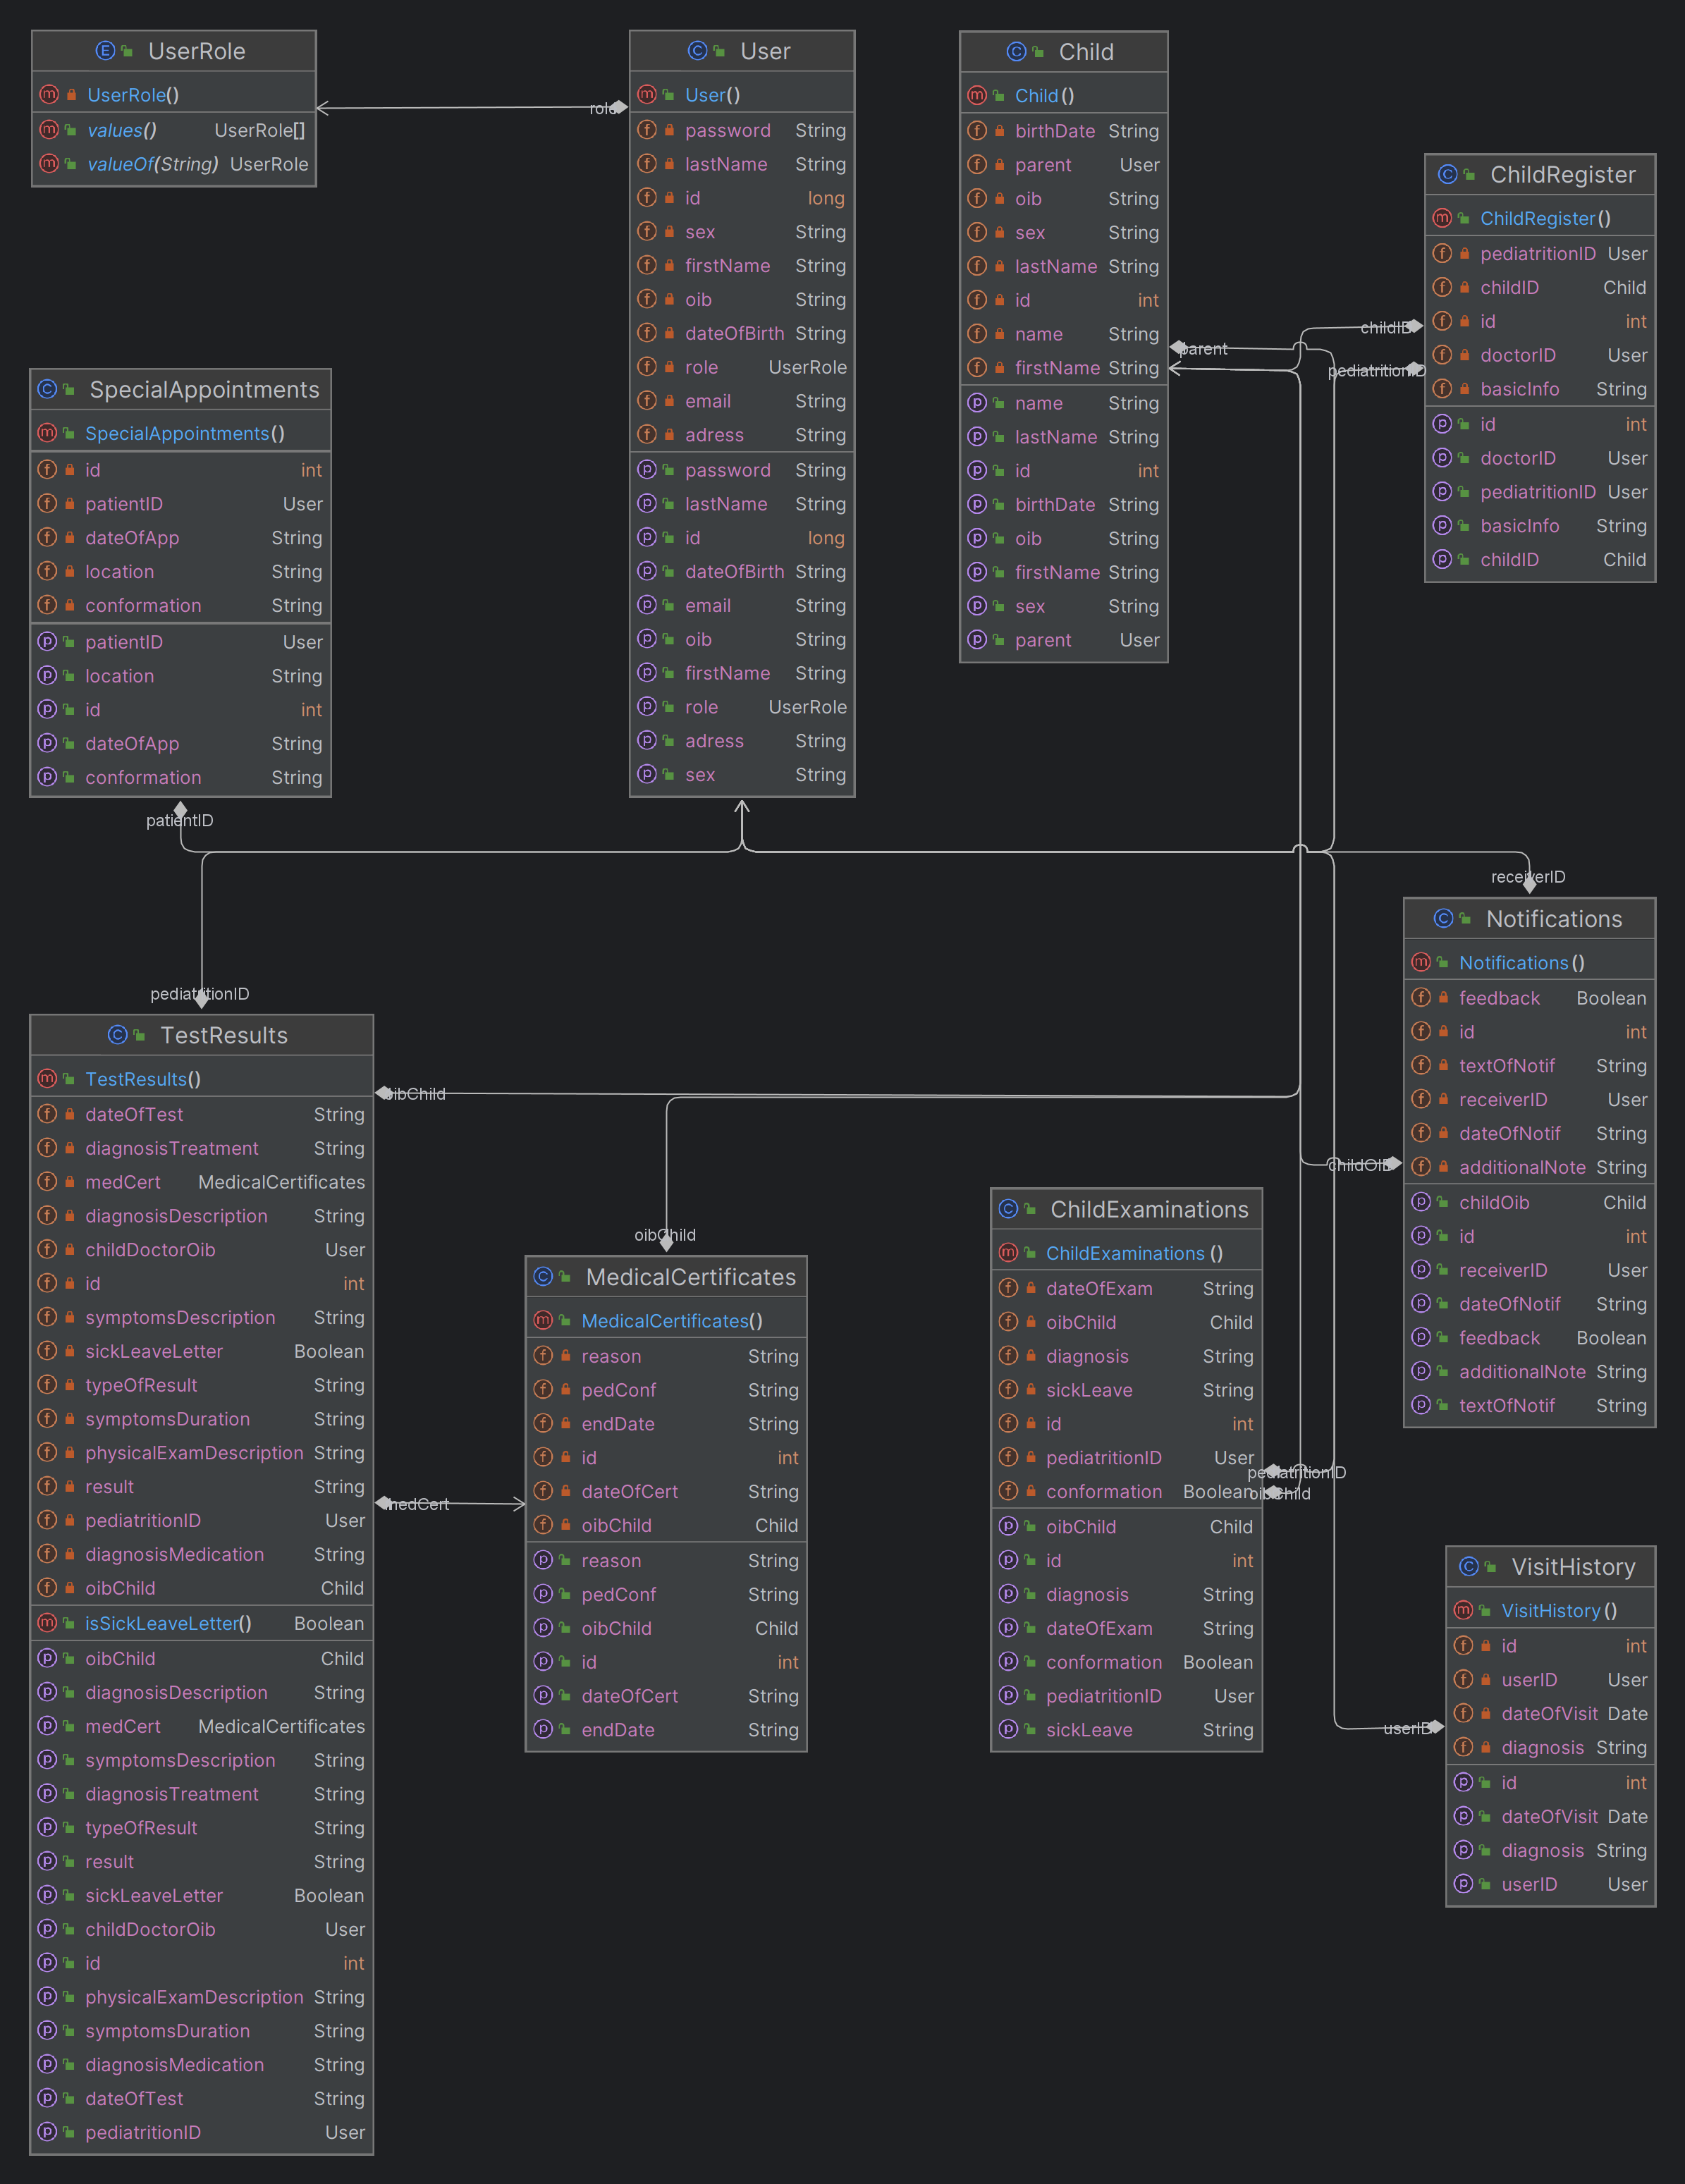
\includegraphics[width=15cm, height=12cm]{dijagrami/class_diagram.png}
			\caption{Dijagram razreda}
			\label{fig:classD}
		\end{figure}
		\eject
		
		\section{Dijagram stanja}
			
			
			\begin{figure}[H]
				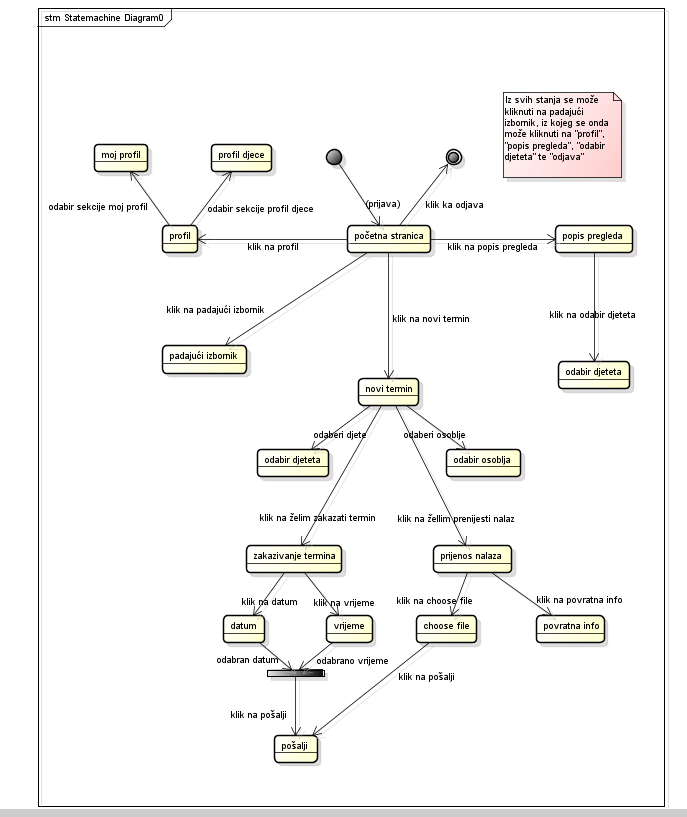
\includegraphics[]{dijagrami/dijagram_stanja.png}
				\caption{Dijagram stanja}
				\label{fig:dijagramStanja}
			\end{figure}
			
			Na priloženom dijagramu stanja prikazano je stanje za prijavljenog korisnika. Nakon prijave korisniku se prikazuje naslovna stranica. Sa naslovne stranice pomoću padajućeg izbornika korisnik može dogovoriti novi termin, pregledati vlastiti profil i popis pregleda te odjaviti se. Klikom na profil prikazuju mu se njegovi podatci ili podatci njegove djece. Klikom na novi termin korisnik može dogovoriti novi termin ili prenijeti dokument u kojem se nalazi njegov nalaz. U svakom trenutku korisnik se preko padajućeg izbornika može vratiti na naslovnu stranicu, odjaviti se te izabrati "profil", "popis pregleda" ili "novi termin".
			
			
			\eject 
		
		\section{Dijagram aktivnosti}
			
			\begin{figure}[H]
				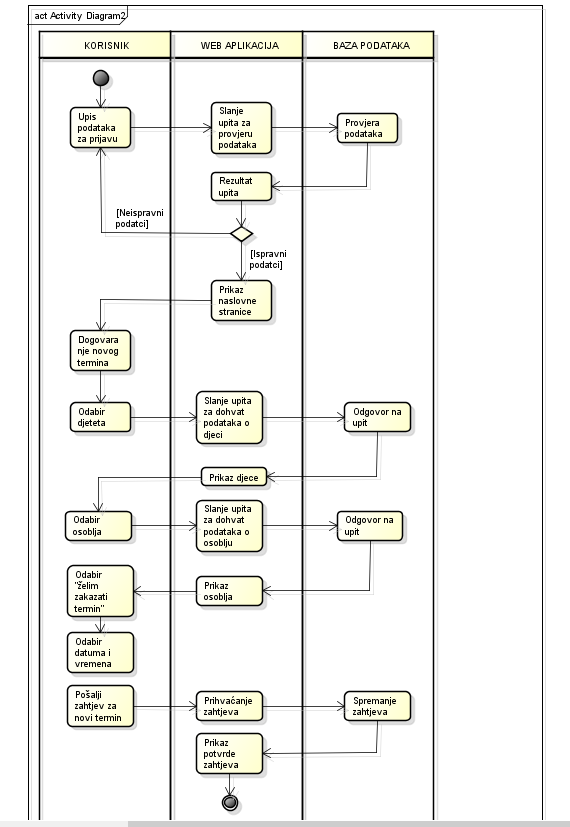
\includegraphics[scale=1.1]{dijagrami/dijagram_aktivnosti.png}
				\centering
				\caption{Dijagram aktivnosti}
				\label{fig:dijagramAktivnosti}
			\end{figure}
			
			Priloženi dijagram aktivnosti prikazuje proces naručivanja na novi termin. Korisnik se prvo prijavi u sustav. Zatim za novi termin odabere djete i osoblje te ispuni datum i vrijeme. Kada je sve od navedenog odabrao te ispunio, korisnik pošalje svoj zahtjev čime on postaje aktivan u sustavu.
			
			\eject
		\section{Dijagram komponenti}
		
			\textbf{\textit{dio 2. revizije}}\\
		
			 \textit{Potrebno je priložiti dijagram komponenti s pripadajućim opisom. Dijagram komponenti treba prikazivati strukturu cijele aplikacije.}

	\chapter{Implementacija i korisničko sučelje}
		
		
		\section{Korištene tehnologije i alati}
		
			\textbf{\textit{dio 2. revizije}}
			
			Za komunikaciju u timu korišten je WhatsApp\footnote{\url{https://www.whatsapp.com/}}. Za pisanje koda korišteni su VSCode\footnote{\url{https://code.visualstudio.com/}} i IntelliJ\footnote{\url{https://www.jetbrains.com/idea/}}. Ovi IDE alati su odabrani radi dobre i kvalitetne implementacije i mogučnosti rada u programskim jezicima odabranim za zadatak, te široke dostupnosti dodataka. Za pisanje dokumentacije korišten je TeXstudio\footnote{\url{https://www.texstudio.org/}} Za izradu UML dijagrama korišteni su AstahUML\footnote{\url{https://astah.net/products/astah-uml/}} i IntelliJ.
			Kao udaljeni repozitorij koda, te za upravljanje zajedničkim razvojem koda korišteni su GitHub\footnote{\url{https://github.com/}} i GitLab\footnote{\url{https://gitlab.com/}}.
			Backend aplikacije pisan je u Javi\footnote{\url{https://www.java.com/en/}} koristeći Springboot\footnote{\url{https://spring.io/projects/spring-boot/}}. Frontend je pisan u Reactu\footnote{\url{https://react.dev/}} i JavaScriptu\footnote{\url{https://www.javascript.com/}}. React je popularana biblioteka u JavaScriptu za izradu korisničkih sučelja. Springboot nudi gotove funkcije i resurse koji omogučuju programerima brži i jednostavniji razvoj backenda.
			Baza Podataka realizirana je PostgreSQL\footnote{\url{https://www.postgresql.org/}}. Za hosting backenda, frontenda i baze podataka korišten je besplatan hosting servis Render\footnote{\url{https://render.com/}}.

			\textit{Detaljno navesti sve tehnologije i alate koji su primijenjeni pri izradi dokumentacije i aplikacije. Ukratko ih opisati, te navesti njihovo značenje i mjesto primjene. Za svaki navedeni alat i tehnologiju je potrebno \textbf{navesti internet poveznicu} gdje se mogu preuzeti ili više saznati o njima}.
			
			\eject 
		
	
		\section{Ispitivanje programskog rješenja}
			
			\textbf{\textit{dio 2. revizije}}\\
			
			 \textit{U ovom poglavlju je potrebno opisati provedbu ispitivanja implementiranih funkcionalnosti na razini komponenti i na razini cijelog sustava s prikazom odabranih ispitnih slučajeva. Studenti trebaju ispitati temeljnu funkcionalnost i rubne uvjete.}
	
			
			\subsection{Ispitivanje komponenti}
			\textit{Potrebno je provesti ispitivanje jedinica (engl. unit testing) nad razredima koji implementiraju temeljne funkcionalnosti. Razraditi \textbf{minimalno 6 ispitnih slučajeva} u kojima će se ispitati redovni slučajevi, rubni uvjeti te izazivanje pogreške (engl. exception throwing). Poželjno je stvoriti i ispitni slučaj koji koristi funkcionalnosti koje nisu implementirane. Potrebno je priložiti izvorni kôd svih ispitnih slučajeva te prikaz rezultata izvođenja ispita u razvojnom okruženju (prolaz/pad ispita). }
			
			
			
\subsection{Ispitivanje sustava}

\textbf{Ispitni slučaj 1: Interakcija s sučeljem za prijavu u sustav}

\noindent \textbf{Ulaz:}
\begin{packed_enum}
	\item Otvaranje početne stranice u web pregledniku.
	\item Unos potrebnim podataka za prijavu u sustav (email i lozinka).
	\item Pritisak na akciju "Prijavi se".
\end{packed_enum}

\noindent \textbf{Očekivani rezultat:}
\begin{packed_enum}
	\item Uspješna prijava korisnika u sustav.
	\item Dolazak na naslovnu stranicu sustava.
\end{packed_enum}

\noindent \textbf{Redovni i rubni slučajevi:}
\begin{packed_enum}
	\item Korisnik je unio ispravan email i lozinku.
	\item Korisnik je unio neispravan email ilil lozinku.
	\item Korisnik nije unio email ili lozinku.
	\item Korisnik nije unio ni email ni lozinku.
\end{packed_enum}

\noindent \textbf{Rezultati:}
\begin{packed_enum}
	\item Korisnik je uspješno prijavljen i doveden na naslovnu stranicu.
	\item Korisnik nije prijavljen i javlja se poruka o neispravnom emailu ili lozinki.
	\item Korisnik nije prijavljen te akcija "Prijavi se" nije dostupna.
	\item Korisnik nije prijavljen te akcija "Prijavi se" nije dostupna.
\end{packed_enum}

\begin{figure}[H]
	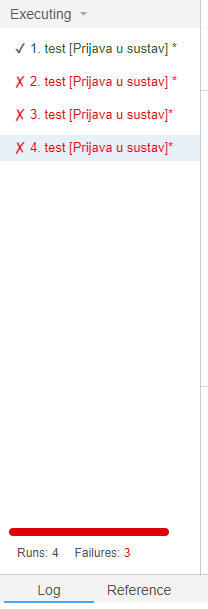
\includegraphics[scale=0.6]{dijagrami/test1.PNG}
	\centering
	\caption{Ispitni slučaj 1. rezultati}
	\label{fig:myChart}
\end{figure}

\begin{figure}[H]
	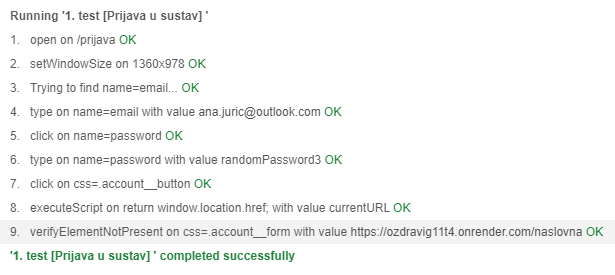
\includegraphics[scale=0.6]{dijagrami/test11.PNG}
	\centering
	\label{fig:myChart}
\end{figure}

\begin{figure}[H]
	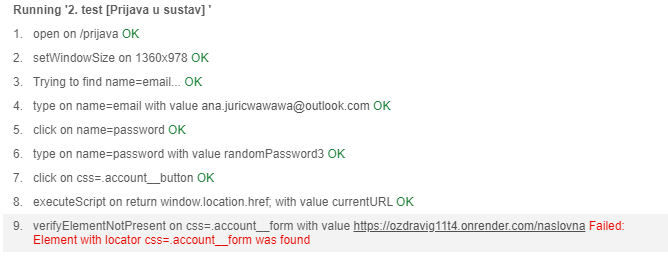
\includegraphics[scale=0.6]{dijagrami/test12.PNG}
	\centering
	\label{fig:myChart}
\end{figure}

\begin{figure}[H]
	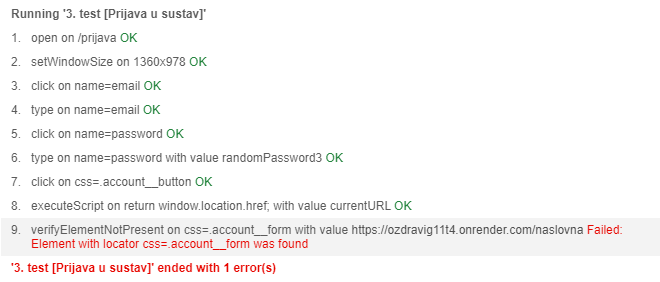
\includegraphics[scale=0.6]{dijagrami/test13.PNG}
	\centering
	\label{fig:myChart}
\end{figure}

\begin{figure}[H]
	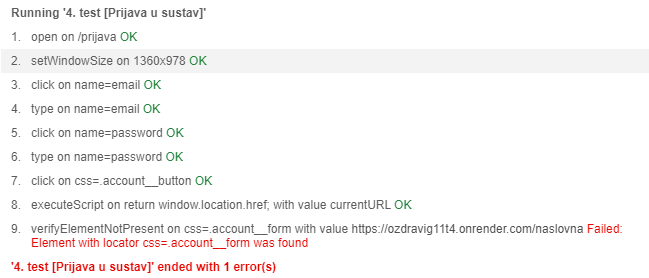
\includegraphics[scale=0.6]{dijagrami/test14.PNG}
	\centering
	\label{fig:myChart}
\end{figure}




\noindent	\textbf{Ispitni slučaj 2: Interakcija s sučeljem za registraciju u sustav}
\\
\noindent \textbf{Ulaz:}
\begin{packed_enum}
	\item Otvaranje početne stranice u web pregledniku.
	\item Unos potrebnim podataka za prijavu u sustav (ime, prezime, email, oib, spol, adresa, lozinka, potvrda lozinke, datum rođenja).
	\item Pritisak na akciju "Registriraj se".
\end{packed_enum}

\noindent \textbf{Očekivani rezultat:}
\begin{packed_enum}
	\item Uspješna registracija korisnika u sustav.
	\item Dolazak na naslovnu stranicu sustava.
\end{packed_enum}

\noindent \textbf{Redovni i rubni slučajevi:}
\begin{packed_enum}
	\item Korisnik je unio ispravne podatke.
	\item Korisnik nije unio sve podatke.
	\item Korisnik je unio neispravni podatak.
	\item Korisnik je unio email ili oib koji već postoji.
\end{packed_enum}

\noindent \textbf{Rezultati:}
\begin{packed_enum}
	\item Korisnik je uspješno registriran i doveden na naslovnu stranicu.
	\item Korisnik nije registriran te akcija "Registriraj se" nije dostupna.
	\item Korisnik nije registriran te akcija "Registriraj se" nije dostupna.
	\item Korisnik nije registriran te se vraća poruka o grešci.
\end{packed_enum}

\begin{figure}[H]
	
\includegraphics[scale=0.6]{dijagrami/test2.PNG}
	\centering
	\caption{Ispitni slučaj 2. rezultati}
	\label{fig:myChart}
\end{figure}

\begin{figure}[H]
	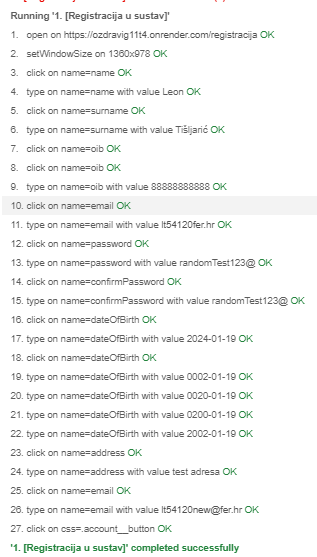
\includegraphics[scale=0.6]{dijagrami/test21.PNG}
	\centering
	\label{fig:myChart}
\end{figure}

\begin{figure}[H]
	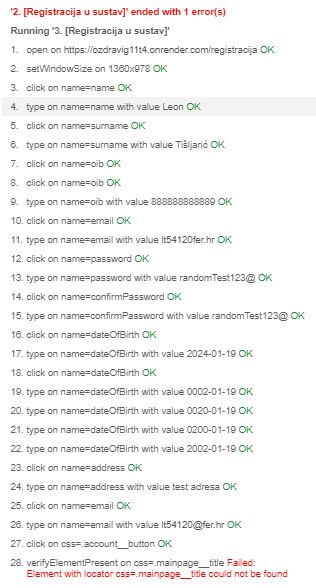
\includegraphics[scale=0.6]{dijagrami/test22.PNG}
	\centering
	\label{fig:myChart}
\end{figure}

\begin{figure}[H]
	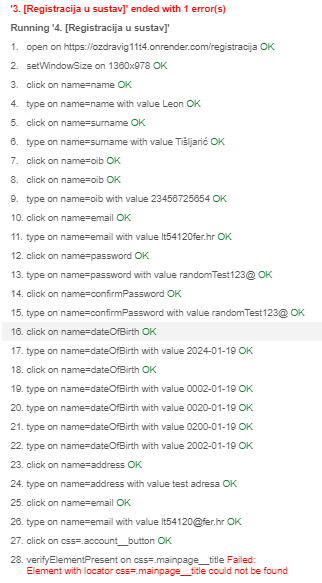
\includegraphics[scale=0.6]{dijagrami/test23.PNG}
	\centering
	\label{fig:myChart}
\end{figure}

\begin{figure}[H]
	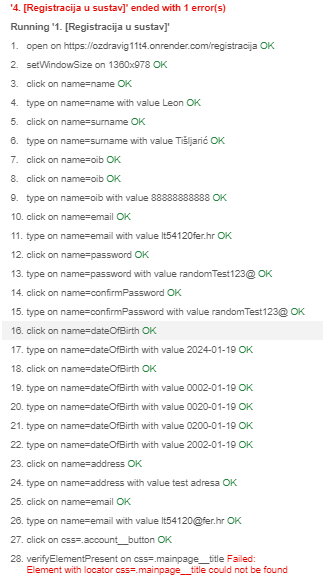
\includegraphics[scale=0.6]{dijagrami/test24.PNG}
	\centering
	\label{fig:myChart}
\end{figure}



\noindent	\textbf{Ispitni slučaj 2: Interakcija s sučeljem roditelja za zakazivanje termina}
\\
\noindent \textbf{Ulaz:}
\begin{packed_enum}
	\item Otvaranje stranice s putanjom "/naslovna/noviTermin".
	\item Odabir dijeteta iz padajućeg izbornika.
	\item Odabir medicinskog osoblja iz padajućeg izbornika.
	\item Odabir opcije "Želim zakazati termin"
	\item Unos datuma i vremena termina
	\item Pritisak na akciju "Pošalji".
\end{packed_enum}

\noindent \textbf{Očekivani rezultat:}
\begin{packed_enum}
	\item Uspješna slanje zahtjeva za novim nalazom.
	\item Prikaz potvrdne poruke o uspješnom slanju.
\end{packed_enum}

\noindent \textbf{Redovni i rubni slučajevi:}
\begin{packed_enum}
	\item Korisnik je unio sve ispravne podatke.
	\item Korisnik nije odabrao dijete ili medicinsko osoblje iz padajućeg izbornika.
	\item Korisnik nije unio datum ili vrijeme.
\end{packed_enum}

\noindent \textbf{Rezultati:}
\begin{packed_enum}
	\item Korisnik je uspješno poslao zahtjev za novim terminom.
	\item Korisnik nije imao mogućnost daljnje ispune zahtjeva za terminom.
	\item Korisnik nije imao mogućnost pokretanja akcije "Pošalji".
\end{packed_enum}

\begin{figure}[H]
	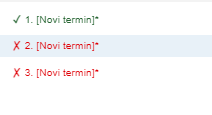
\includegraphics[scale=0.6]{dijagrami/test3.PNG}
	\centering
	\caption{Ispitni slučaj 3. rezultati}
	\label{fig:myChart}
\end{figure}

\begin{figure}[H]
	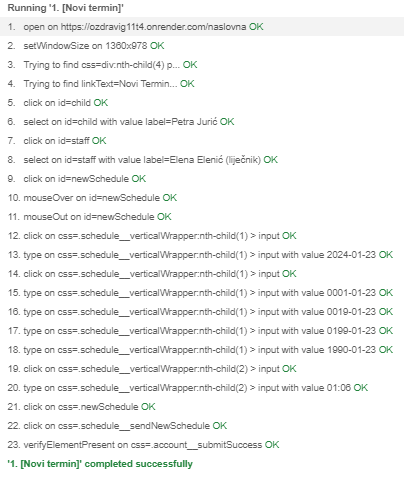
\includegraphics[scale=0.6]{dijagrami/test31.PNG}
	\centering
	\label{fig:myChart}
\end{figure}

\begin{figure}[H]
	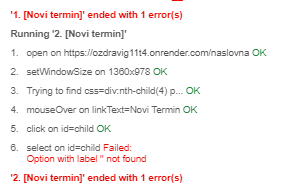
\includegraphics[scale=0.6]{dijagrami/test32.PNG}
	\centering
	\label{fig:myChart}
\end{figure}

\begin{figure}[H]
	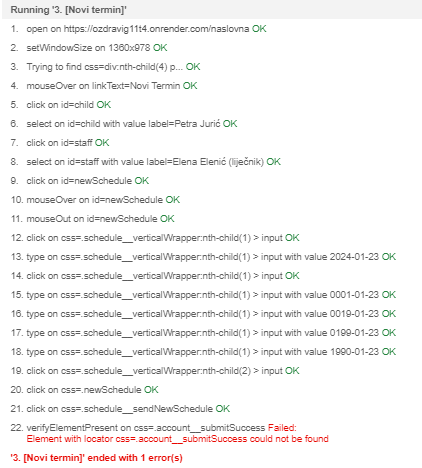
\includegraphics[scale=0.6]{dijagrami/test33.PNG}
	\centering
	\label{fig:myChart}
\end{figure}



\noindent	\textbf{Ispitni slučaj 4: Interakcija s sučeljem roditelja za slanje nalaza}
\\
\noindent \textbf{Ulaz:}
\begin{packed_enum}
	\item Otvaranje stranice s putanjom "/naslovna/noviTermin".
	\item Odabir dijeteta iz padajućeg izbornika.
	\item Odabir medicinskog osoblja iz padajućeg izbornika.
	\item Odabir opcije "Želim prenijeti nalaz"
	\item Prijenos datoteke
	\item Pritisak na akciju "Pošalji".
\end{packed_enum}

\noindent \textbf{Očekivani rezultat:}
\begin{packed_enum}
	\item Uspješna slanje i pohrana nalaza u sustav.
	\item Prikaz potvrdne poruke o uspješnom slanju.
\end{packed_enum}

\noindent \textbf{Redovni i rubni slučajevi:}
\begin{packed_enum}
	\item Korisnik je unio sve ispravne podatke.
	\item Korisnik nije odabrao dijete ili medicinsko osoblje iz padajućeg izbornika.
	\item Korisnik nije unio nalaz za prijenos.
\end{packed_enum}

\noindent \textbf{Rezultati:}
\begin{packed_enum}
	\item Korisnik je uspješno poslao zahtjev za novim terminom.
	\item Korisnik nije imao mogućnost daljnje ispune zahtjeva za terminom.
	\item Korisnik nije imao mogućnost pokretanja akcije "Pošalji".
\end{packed_enum}


\eject 
		
		
		\section{Dijagram razmještaja}
			
			\textbf{\textit{dio 2. revizije}}
			
			 \textit{Na poslužiteljskom računalu se nalaze web poslužitelj i poslužitelj baze podataka. Korisnici koriste web preglednik za pristup web aplikaciji. Sustav je baziran na arhitekturi ”klijent – poslužitelj”, a komunikacija između računala korisnika i poslužitelja odvija se preko HTTP veze.}
			
			\begin{figure}[H]
				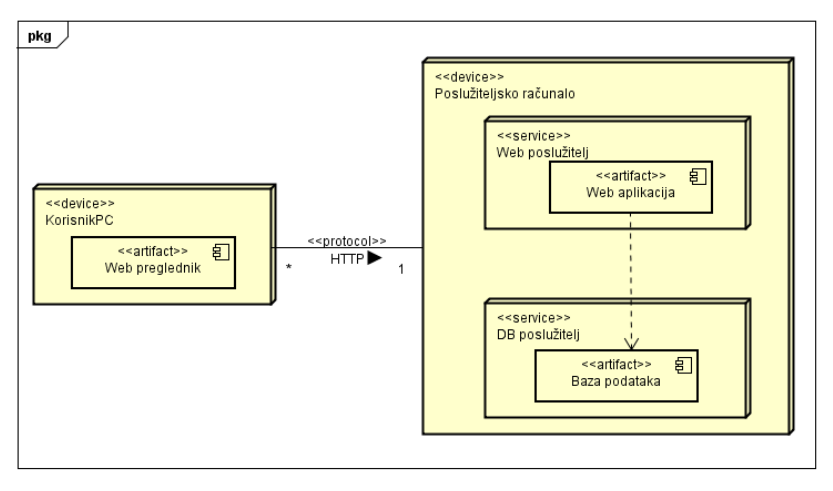
\includegraphics[width=15cm, height=12cm]{dijagrami/dijagram_razmjestaja.png}
				\caption{Dijagram razmještaja}
				\label{fig:classD}
			\end{figure}
			
			\eject 
		
		\section{Upute za puštanje u pogon}
		
			\textbf{\textit{dio 2. revizije}}\\
		
			 \textit{U ovom poglavlju potrebno je dati upute za puštanje u pogon (engl. deployment) ostvarene aplikacije. Na primjer, za web aplikacije, opisati postupak kojim se od izvornog kôda dolazi do potpuno postavljene baze podataka i poslužitelja koji odgovara na upite korisnika. Za mobilnu aplikaciju, postupak kojim se aplikacija izgradi, te postavi na neku od trgovina. Za stolnu (engl. desktop) aplikaciju, postupak kojim se aplikacija instalira na računalo. Ukoliko mobilne i stolne aplikacije komuniciraju s poslužiteljem i/ili bazom podataka, opisati i postupak njihovog postavljanja. Pri izradi uputa preporučuje se \textbf{naglasiti korake instalacije uporabom natuknica} te koristiti što je više moguće \textbf{slike ekrana} (engl. screenshots) kako bi upute bile jasne i jednostavne za slijediti.}
			
			
			 \textit{Dovršenu aplikaciju potrebno je pokrenuti na javno dostupnom poslužitelju. Studentima se preporuča korištenje neke od sljedećih besplatnih usluga: \href{https://aws.amazon.com/}{Amazon AWS}, \href{https://azure.microsoft.com/en-us/}{Microsoft Azure} ili \href{https://www.heroku.com/}{Heroku}. Mobilne aplikacije trebaju biti objavljene na F-Droid, Google Play ili Amazon App trgovini.}
			
			
			\eject 

	\chapter{Zaključak i budući rad}
		
		\textbf{\textit{dio 2. revizije}}\\

			Zadatak našeg tima bio je razvoj web aplikacije koja olakšava komunikaciju, rezervaciju termina pregleda, te prosljeđivanje uputnica i ispričnica između doktora, roditelja i škola. Nakon nešto manje od četiri mjeseca razvoja, ovo je večinski ostvareno kroz dvije faze razvoja.
			
			Prva faza započela je okupljanjem članova tima i dodjelom projektnog zadatka. Tijekom prve faze započeli smo fokusom na konceptualnu razradu implementacije aplikacije - njenog korisničkog sučelja, baze podataka, te omogučenih funkcionalnosti svakog tipa korsinika.
			Slijedila je edukacija svih članova tima o tehnologijama Springboot i React putem prisutstvovanja na stručnim predavanjima CROZ-a, te samostalnim radom.
			Nakon razrade koncepcije aplikacije i upoznavanja s tehnologijama krenuli smo u implementaciju sa fokusom na razvoj korisničkog sučelja aplikacije, te uspostave funkcionalne baze podataka dogovorene arhitekture. Kada je baza bila uspostavljena, backend tim je krenuo u početne faze povezivanja korisničkog sučelja na bazu, dok se frontend tim prebacio na dokumentaciju.
			Deployem aplikacije na servis "onrender" završila je prva faza.

			Druga faza je po pitanju kodiranja bila intenzivnija od prve. Zahvaljujući dobrim rješenjima korijenitih aspkeata aplikacije u prvoj fazi, druga je faza mogla biti puno više fokusirana na implementaciju traženih funkcionalnosti.
			Neovisan pristup razvoja frontenda i backenda uz naglasak na komunikaciju i držanje dogovorene arhitekture omogučio je brz razvoj, pri tom zadržavajući konzistentnost i lagano spajanje implementiranoga.
			Fokus druge faze bio je dovršetak korisničkog sučelja, te povezivanje istog na backend. Kasnije razdoblje faze fokusiralo se na pisanje dokumentaicje, testiranje i bugfixing.

			Od samog početka rada na zadatku, naš tim je naišao na svoj prvi izazov - nemogučnost sudjelovanja dva člana. Ovaj izazov je u dogovoru s CROZ-om i profesorima predmeta riješen dogovorenim izostavljanjem dva zahtjeva implementacije:
			\begin{itemize}
				\item Roditelji dobivaju obavijest/uputu od pedijatra ili liječnik obiteljske medicine nakon što je stigao nalaz iz laboratorija
				\item Liječnik obiteljske medicine ili pedijatar naručuje pacijenta na specijalistički pregled / postupak, a pacijent dobiva poruku s potvrdom o naručivanju s prikazom lokacija na mapi gdje taj pregled može obaviti s obzirom na mjesto stanovanja (OpenStreetMap)
			\end{itemize}
			Ovo smanjenje ljudstva je rezultiralo nešto sporijim razvojem i pisanjem dokumentacije, te potrebom članova da rade na više djelova projekta. Tako su članovi frontend podtima povremeno radili na backendu i obrnuto, te je cijeli tim bio zadužen za pisanje dokumentacije, umjesto jednog člana kojemu bi to bio primarni fokus.
			Unatoč navedenom, uspješno smo implementirani dogovorene zahtjeve u roku.
			Očekivali smo popriličan izazov u nepoznavanju tehnologija korištenih za razvoj aplikacije, no ispostavilo se kako su ih članovi tima brzo naučili i stvorili mogučnost razvoja u njima. Jedna dobra posljedica nedostatka članova u timu bila je i bolja upoznatost svih članova sa svim korištenim tehnologijama.
			
			Komunikacija između članova tima bila je ostvarena putem WhatsApp grupe što je omogučilo efektivnu i brzu razmjenu informacija.
			Ona se pokazala kao iznimno korisna, te je rezultirala dobrom standardizacijom koda i uspješnim držanjem dogovorenih normi i koncepata.
			Tim je cijelo razdoblje rada na aplikaciji proveo dobro informiran u vezi djelovanja ostalih članova tima.

			Naša preporuka za daljnji razvoj apliakcije bila bi implementacija mogučnosti koje smo mi morali izostaviti. Vjerujemo kako bi rezultirale kvalitetnijim korisničkim iskustvom.
			Također je moguć razvoj mobilne aplikacije koja bi mogla kvalitetnije implementirati notifikacije, te pružiti opećenito ugodnije korisničko iskustvo nego web preglednik.
			Za kraj, preporučili bi i razvoj jednostavnog chat-featurea za direktnu komunikaciju između doktora i roditelja.

			Rad na ovom projektu nam je dao nekoliko neprocijenjivih iskustava. Prije svega iskustvo timskog rada koje će svakome od nas biti neprocijenjivo u daljnjoj karijeri.
			Iskustvo "on-the-fly" učenja tehnologija je članovima pokazalo njihovu mogučnost brzog snalaženja. Naš početni izazov rezultirao je i sticanjem iskustva snalaženja u neočekivanim okolnostima, no još je bitnije unutar tima stvorio kulturu proaktivnog "uskakanja" u pomoć drugim članovima.
			Konačno, svi članovi tima su ovim projektom stekli znanje i iskustvo u često korištenim tehnologijama, te iskustvo potpunog razvoja projekta od svojeg početka do kraja.

		\eject 

	\chapter*{Popis literature}
		\addcontentsline{toc}{chapter}{Popis literature}

		\begin{enumerate}
			
			
			\item  Programsko inženjerstvo, FER ZEMRIS, \url{http://www.fer.hr/predmet/proinz}
			
			\item  The Unified Modeling Language, \url{https://www.uml-diagrams.org/}
			
		\end{enumerate}
		
		 
	
	
	\begingroup
	\renewcommand*\listfigurename{Indeks slika i dijagrama}
	%\renewcommand*\listtablename{Indeks tablica}
	%\let\clearpage\relax
	\listoffigures
	%\vspace{10mm}
	%\listoftables
	\endgroup
	\addcontentsline{toc}{chapter}{Indeks slika i dijagrama}


	
	\eject 
		
	\chapter*{Dodatak: Prikaz aktivnosti grupe}
		\addcontentsline{toc}{chapter}{Dodatak: Prikaz aktivnosti grupe}
		
		\section*{Dnevnik sastajanja}
		
		\begin{packed_enum}
			\item  sastanak
			
			\item[] \begin{packed_item}
				\item Datum: 23. listopada 2023.
				\item Prisustvovali: Hrvoje Cerin, Leon Tišljarić, Matko Ljepović,  Šimun Banović
				\item Teme sastanka:
				\begin{packed_item}
					\item  Raspodjela poslova
					\item  Upoznavanje članova tima
					\item  Nazočnost na CROZ predavanju
				\end{packed_item}
			\end{packed_item}
			
			\item  sastanak
			\item[] \begin{packed_item}
				\item Datum: 9. studenoga 2023.
				\item Prisustvovali: Hrvoje Cerin, Leon Tišljarić, Matko Ljepović,  Dan Široki
				\item Teme sastanka:
				\begin{packed_item}
					\item  Dogovor vezani uz implementaciju stavki
					\item  Proučavanje primjera dokumentacije
					\item  Nazočnost na CROZ predavanju
				\end{packed_item}
			\end{packed_item}
			
			%
			
		\end{packed_enum}
		
		\eject
		\section*{Tablica aktivnosti}
		
			\textbf{\textit{Kontinuirano osvježavanje}}\\
			
			 \textit{Napomena: Doprinose u aktivnostima treba navesti u satima po članovima grupe po aktivnosti.}

			\begin{longtblr}[
					label=none,
				]{
					vlines,hlines,
					width = \textwidth,
					colspec={X[7, l]X[1, c]X[1, c]X[1, c]X[1, c]X[1, c]X[1, c]X[1, c]}, 
					vline{1} = {1}{text=\clap{}},
					hline{1} = {1}{text=\clap{}},
					rowhead = 1,
				} 
			
				\SetCell[c=1]{c}{} & \SetCell[c=1]{c}{\rotatebox{90}{\textbf{Hrvoje Cerin}}} & \SetCell[c=1]{c}{\rotatebox{90}{\textbf{Leon Tišljarić }}} &	\SetCell[c=1]{c}{\rotatebox{90}{\textbf{Dan Široki }}} & \SetCell[c=1]{c}{\rotatebox{90}{\textbf{Matko Ljepović }}} &	\SetCell[c=1]{c}{\rotatebox{90}{\textbf{Šimun Banović }}} & \SetCell[c=1]{c}{\rotatebox{90}{\textbf{-}}} &	\SetCell[c=1]{c}{\rotatebox{90}{\textbf{-}}} \\  
				Upravljanje projektom 		&x  &  &  &  &  &  & \\ 
				Opis projektnog zadatka 	&  &x  &  &  &  &  & \\ 
				
				Funkcionalni zahtjevi       &x  &x  &x  &x  &x  &  &  \\ 
				Opis pojedinih obrazaca 	&  &  &  &  &  &  &  \\ 
				Dijagram obrazaca 			&  &  &  &  &  &  &  \\ 
				Sekvencijski dijagrami 		&  &  &  &  &  &  &  \\ 
				Opis ostalih zahtjeva 		&  &  &  &  &  &  &  \\ 

				Arhitektura i dizajn sustava	 &x  &x  &  &  &x  &  &  \\ 
				Baza podataka				&x  &  &  &x  &x  &  &   \\ 
				Dijagram razreda 			&  &  &  &  &x  &  &   \\ 
				Dijagram stanja				&  &  &x  &  &  &  &  \\ 
				Dijagram aktivnosti 		&  &  &x  &  &  &  &  \\ 
				Dijagram komponenti			&  &  &  &  &  &  &  \\ 
				Korištene tehnologije i alati 		&  &  &  &  &  &  &  \\ 
				Ispitivanje programskog rješenja 	&  &  &  &  &  &  &  \\ 
				Dijagram razmještaja			&  &  &x  &  &  &  &  \\ 
				Upute za puštanje u pogon 		&  &  &  &  &  &  &  \\  
				Dnevnik sastajanja 			&  &  &  &  &  &  &  \\ 
				Zaključak i budući rad 		&  &  &  &  &  &  &  \\  
				Popis literature 			&  &  &  &  &  &  &  \\  
				&  &  &  &  &  &  &  \\ \hline 
				\textit{Dodatne stavke} 			&  &  &  &  &  &  &  \\ 
				\textit{Front end}		&  &x  &x  &  &  &  &  \\
				\textit{Izrada početne stranice} 				&  &x  &x  &  &  &  &  \\  
				\textit{Izrada side bar-a} 				&  &x  &  &  &  &  &  \\  
				\textit{Izrada stranice za login i registraciju} 				&  &x  &  &  &  &  &  \\  
				\textit{Back end} 							&x  &  &  &x  &x  &  &  \\  
				\textit{Izrada baze podataka} 		 			&x  &  &  &x  &x  &  & \\  
				\textit{Spajanje s bazom podataka} 							&x  &x  &  &x  &x  &  &  \\ 
				\textit{Deployment}		&x	&	&	&	&	&	&\\
				 							&  &  &  &  &  &  &\\ 
			\end{longtblr}
					
					
		\eject
		\section*{Dijagrami pregleda promjena}
			\begin{figure}
				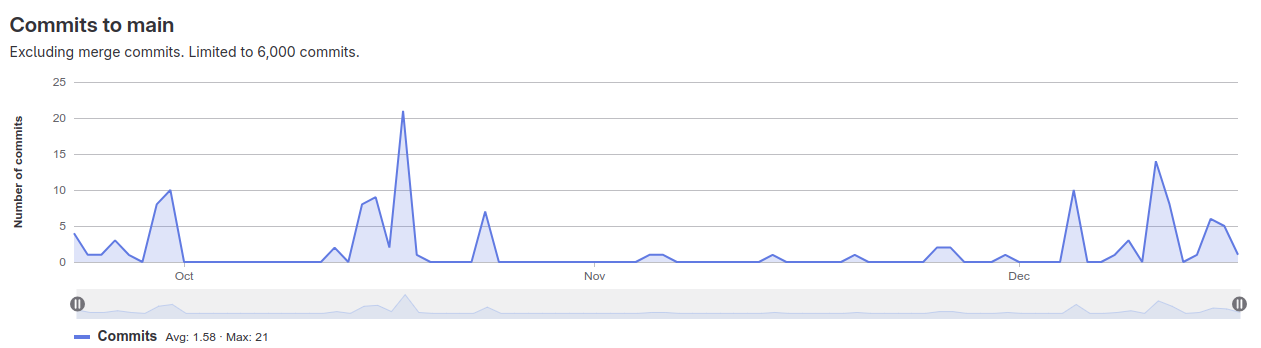
\includegraphics[width=15cm]{dijagrami/dijagram_pregleda_promjena.png}
			\end{figure}
			\begin{figure}
				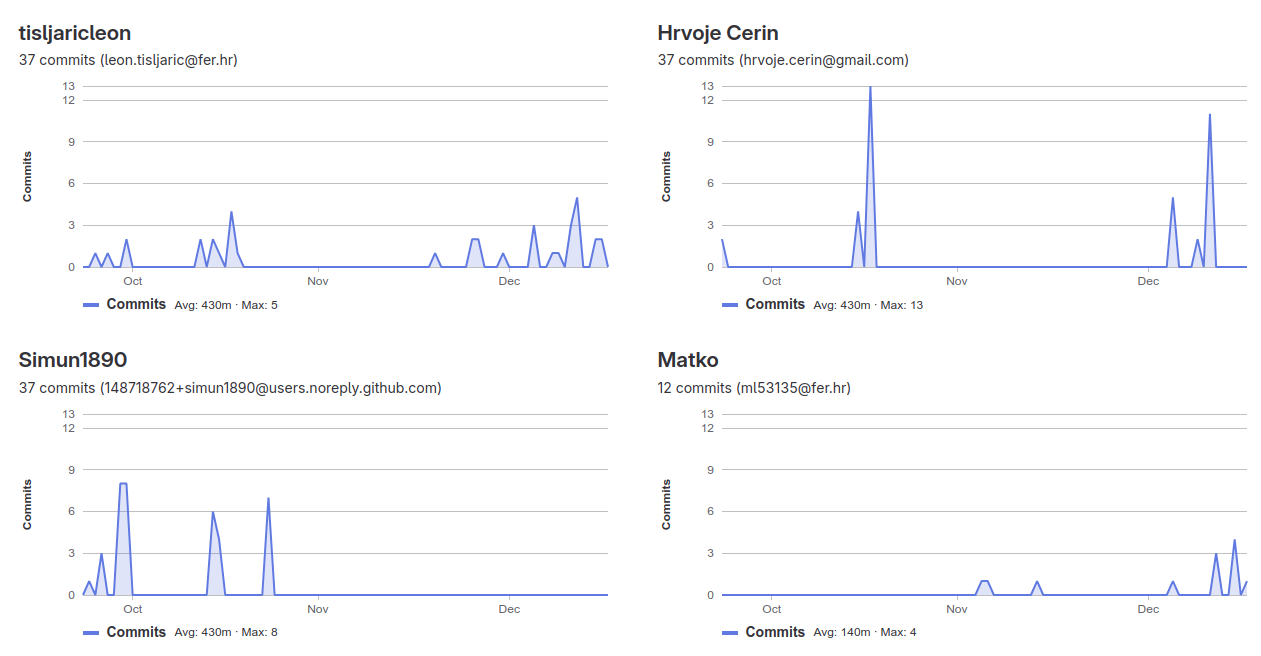
\includegraphics[width=15cm]{dijagrami/dijagram_pregleda_promjena2.png}
			\end{figure}
			\begin{figure}
				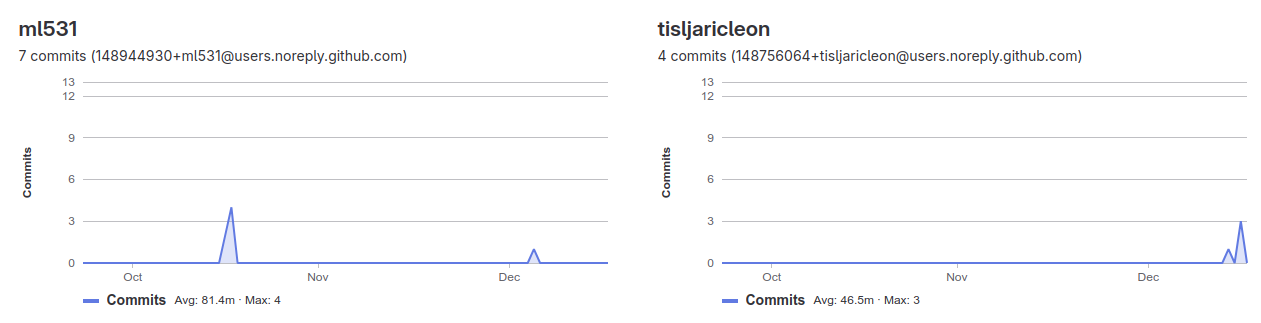
\includegraphics[width=15cm]{dijagrami/dijagram_pregleda_promjena3.png}
			\end{figure}
			\textit{Prenijeti dijagram pregleda promjena nad datotekama projekta. Potrebno je na kraju projekta generirane grafove s gitlaba prenijeti u ovo poglavlje dokumentacije. Dijagrami za vlastiti projekt se mogu preuzeti s gitlab.com stranice, u izborniku Repository, pritiskom na stavku Contributors.}
		\eject
		
	



\end{document} %naredbe i tekst nakon ove naredbe ne ulaze u izgrađen dokument 


